
\section{Material and methods}

\subsection{Simulation setup}\label{SimuSetup}

The monitoring system modeled in this simulation work is the Compton camera prototype under development within the French collaboration CLaRyS. The detectors detailed characteristics can be found in \cite{krimmer:hal-01101334}.\\
%Like most of the Compton camera devices, the CLaRyS prototype includes a scatterer and an absorber. 
The scatterer consists of seven parallel planes of silicon detectors (double-sided silicon strip detectors, DSSDs), $9\times9\times0.2$~cm$^3$, with 1~cm distance between the centers of two neighboring planes, while the absorber is composed of an array of $10\times10$ BGO (Bismuth Germanate - Bi$_{12}$GeO$_{20}$) blocks ($3.5\times3.5\times3.0$~cm$^3$ each) placed behind the silicon layers at a distance which can be tuned according to the requirements.

\begin{figure}	
  \centering
  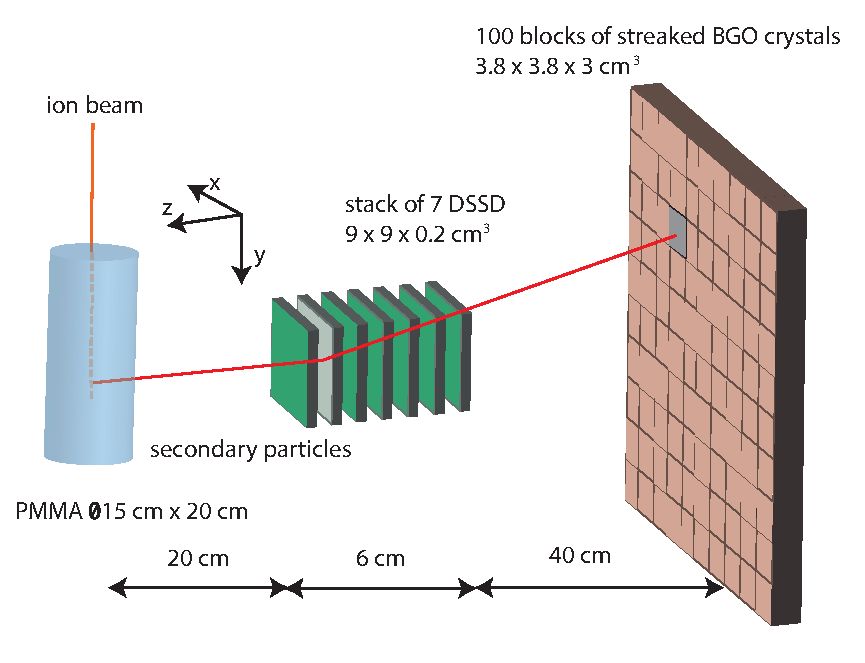
\includegraphics[width=0.7\textwidth]{./Figure/Compton_Camera_hadontherapy_PMMA_Cylinder_EN.pdf}
  \caption{Scheme of the simulation setup (not at scale): a PMMA cylindrical phantom is set in front of the Compton camera prototype. The Compton camera is composed of a stack of 7 double sided silicon strip detectors (scatterer) and a plane of 100 single BGO blocks. The set distances are realistic for clinical conditions. This geometrical configuration has been used for all the simulations presented in this work.}
  \label{fig:fig_setup_CC_simulation_Hadronth}
\end{figure}

The silicon detectors have a strip pitch of 1.4~mm, for a total of 64 strips per side (double-sided readout based on electron and hole pairs collection). 
Regarding the BGO blocks, their entrance surface is streaked in a 8$\times$8 matrix of pseudo-pixels, $4.4\times4.4$~mm$^{2}$ size, and the readout is performed via 4 photo-multiplier tubes. The position reconstruction is achieved via Anger logic~\cite{Fontana2018}.

A scheme of the simulation setup is given in figure~\ref{fig:fig_setup_CC_simulation_Hadronth}. The ion beam interacts with a cylindrical PMMA (PolyMethylMethAcrylate) phantom (15~cm diameter and 20~cm length) placed in front of the Compton camera as target. It is placed 20~cm far from the first silicon plane (center-to-center distance) which seems a realistic distance in clinical conditions. The distance between the last silicon layer and the absorber array (center-to-center) is set to 40~cm in order to enable time-of-flight measurements (see section~\ref{MatMeth::TOF_Ecut}).

The silicon detector strips are not reproduced in the simulation code, and the spatial resolution in the detector plane is set to 0.9~mm FWHM at the reference energy of 1~MeV, according to preliminary measurements performed on smaller detector prototypes. In the plane of the detectors (xy in figure~\ref{fig:fig_setup_CC_simulation_Hadronth}), interactions are defined as localized energy deposits, and the events presenting multiple hits separated by a distance beyond 3-strip equivalent are rejected. For the accepted multiple-hit interactions, the interaction position in the detector plane is defined as the center of gravity of the hits, weighted with the hit energy deposit. Concerning the direction perpendicular to the detector plane (z axis in figure~\ref{fig:fig_setup_CC_simulation_Hadronth}), the interaction position is set to the center of the involved silicon plane. A mono-block crystal is simulated for the absorber for simplicity. The events are selected to be limited to a single block component based on the interaction localization, and, as for the scatterer layers, the interaction position is reconstructed via center of gravity calculation if multiple interactions occur within the same block. An uncertainty contribution, randomly extracted by a Gaussian of 5~mm FWHM (corresponding to an overestimation of the geometrical resolution given by the pseudo-pixel matrix, set to reproduce not yet tested experimental conditions), is added to the reconstructed position to mimic the pseudo-pixel-based readout. For what concerns the z direction, given the fact that the employed BGO blocks have not depth of interaction reconstruction capabilities, the interaction position is fixed to the center of the mono-block crystal.

The energy resolution of the silicon detector is set to 5~keV (FWHM) for an energy deposit of 200~keV according to the design expectations, and varies as a function of $\sqrt{E_{1}}$.
The energy resolution of the BGO blocks was estimated in preliminary measurements and is accordingly set to 20\% FWHM at the reference energy of 667~keV (a 137-cesium source has been used for the measurements). 

The time resolution has been set to 15.0~ns FWHM for the silicon slabs and to 3.0~ns FWHM for the BGO blocks, according to preliminary measurements performed on test detector modules at the GANIL center in France.

The detector resolutions play an important role in the Compton camera performances. The spatial resolution of the absorber influences the axis orientation of the Compton cone. The energy resolution of the scatterer determines the Compton cone aperture angle. The time resolution impacts the coincidence window between the absorber and the scatterer, and therefore the detectors ability to distinguish between true and random coincidences.

The CLaRyS project also includes the development of a beam tagging hodoscope, composed of scintillating fibers read out by multi-channel photomultipliers. This detector is used to synchronize the beam time and space structure to the prompt gamma detection in order to tune the detection window reducing the background contamination. In addition to this, the spatial localization of the impinging beam bunch can be included in the event reconstruction algorithm to add constraints to the obtained solutions (see section~\ref{MatMeth:reconstruction}). The hodoscope is not included in the simulation, but its spatial and time resolution have to be taken into account for the time-of-flight discrimination (see section~\ref{MatMeth::TOF_Ecut}) and events reconstruction. They are set to 1~ns and 1~mm FWHM, respectively.\\ 
The detector's spatial, energy, and time resolutions are summarized in table \ref{table:table_resolution_detecteurs_CC_simulation_Hadronth}.

\begin{table}
\centering
%\begin{tabular}{>{\columncolor[gray]{0.9}}ccc}
\caption{Estimations of reachable resolutions with the detectors. Those resolutions are applied during the simulations.}
\begin{tabular}{cccc}
\hline
\textbf{Resolution (FWHM) at 1~MeV} & \textbf{Scatterer} & \textbf{Absorber} & \textbf{Hodoscope}\\
\hline 
\textbf{spatial [mm]	}			 &     0.9		 &  5 &	 1\\
%\hline
\textbf{energy}				&	5~keV		&  17~\%	&	/\\
%\hline
\textbf{timing [ns]}	        		&	15			&	3 	&  1\\
\hline
\end{tabular}
\label{table:table_resolution_detecteurs_CC_simulation_Hadronth}
\end{table}
    
The Monte Carlo simulation is performed with the Geant4 toolkit, version 9.6.02. 
%Geant4 has been developed at CERN %(Conseil europ\'{e}en pour la recherche nucl\'{e}aire) for high energy physics experiments, but it has been shown that it can be used for ion beam therapy studies \cite{cirrone_hadrontherapy_2011,toshito_new_2010}. 
%Some improvements are still needed in order to extend the hadronic models to low energy applications~\cite{dedes_assessment_2014, Pinto:2016aa}.
The particle interactions in matter are described in this work by means of the models listed in table~\ref{table:table_modele_physic_CC_simulation_Hadronth}. Additionally, the Doppler broadening and the photon polarization effects are included.
 

\definecolor{Gray}{gray}{0.9}

\begin{table}
\label{physlist_ion}
\caption{Hadronic models used in the Geant4 simulations.}
%\begin{scriptsize}
\begin{center}
%\renewcommand{\arraystretch}{1.2}
\resizebox{\textwidth}{!}{%
%\begin{tabular} {>{\columncolor[gray]{0.9}}cccc}\hline  
\begin{tabular} {cccc}\hline
%\rowcolor{Gray}
\textbf{Process} & \textbf{Protons} & \textbf{Ions} & \textbf{Neutrons} \\ \hline 
\textbf{Electromagnetic} & \multicolumn{3}{c}{standard$_{\rm{option3}}$} \\ %\hline
\textbf{Inelastic} & G4BinaryCascade & G4QMDReaction  &  G4BinaryCascade  \\ 
 & & (G4IonsShenCrossSection)&+ G4NeutronHPInelastic ($<$19~MeV)\\ %\hline
\textbf{Elastic} & G4LElastic & G4LElastic & G4LElastic + G4NeutronHPElastic ($<$19~MeV)\\ %\hline
\textbf{Fission} & / & / & G4LFission + G4NeutronHPFission($<$19~MeV) \\ %\hline
\textbf{Capture} & / & / & G4LCapture +  G4NeutronHPCapture ($<$19~MeV) \\ %\hline
\textbf{Radioactivedecay} & / & G4Radioactivedecay & / \\ \hline
\end{tabular}}
\end{center}
%\end{scriptsize}
\label{table:table_modele_physic_CC_simulation_Hadronth}
\end{table}

%\subsection{Data processing}
%\label{subsection:Treatment_data_CC_hadrontherapy_Geant4}

\subsection{Beam structure}
\label{subsection:modelisation_fasceau_ions_CC_hadrontherapy_Geant4}
\subsubsection{Beam structure measurements at HIT}\label{beam_measurement}
Our group performed a set of measurements to characterize the beam time structure of the synchrotron installed in the Heidelberg Ion Therapy Center (HIT), Germany~\cite{HIT_timestructure}. This set of measurements extends the results reported in~\cite{HIT_timestructure} and is then used to reproduce a realistic beam in the simulation.\\
The beam characterization has been performed for 200~MeV/u and 400~MeV/u primary carbon ion energy with a two-fiber hodoscope (basic prototype of the one at present under development) and the spill signal was given by the accelerator. Figure \ref{fig:fig_structure_temps_faisceau_HIT_2013_CC_simulation_Hadronth} shows the results for carbon ions at 400~MeV/u. The pulses have a spill period of 150.2~ns and each bunch is approximately 21.5~ns.
The mentioned measurements have shown that the spill phase changes during the extraction: this implies that the HF signal from the synchrotron can not be used to trigger the pulses, so that the use of an additional beam time stamp system like the hodoscope seems required for time-of-flight background rejection purposes.

\begin{figure} [!hbtp]	
  \centering
  %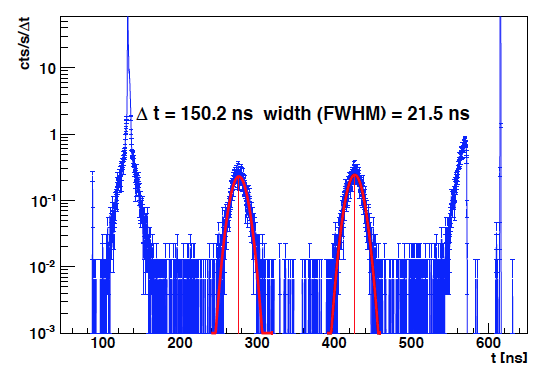
\includegraphics[width=0.6\textwidth]{./Figure/2013_Structure_Time_Beam_400MeV.png}
  %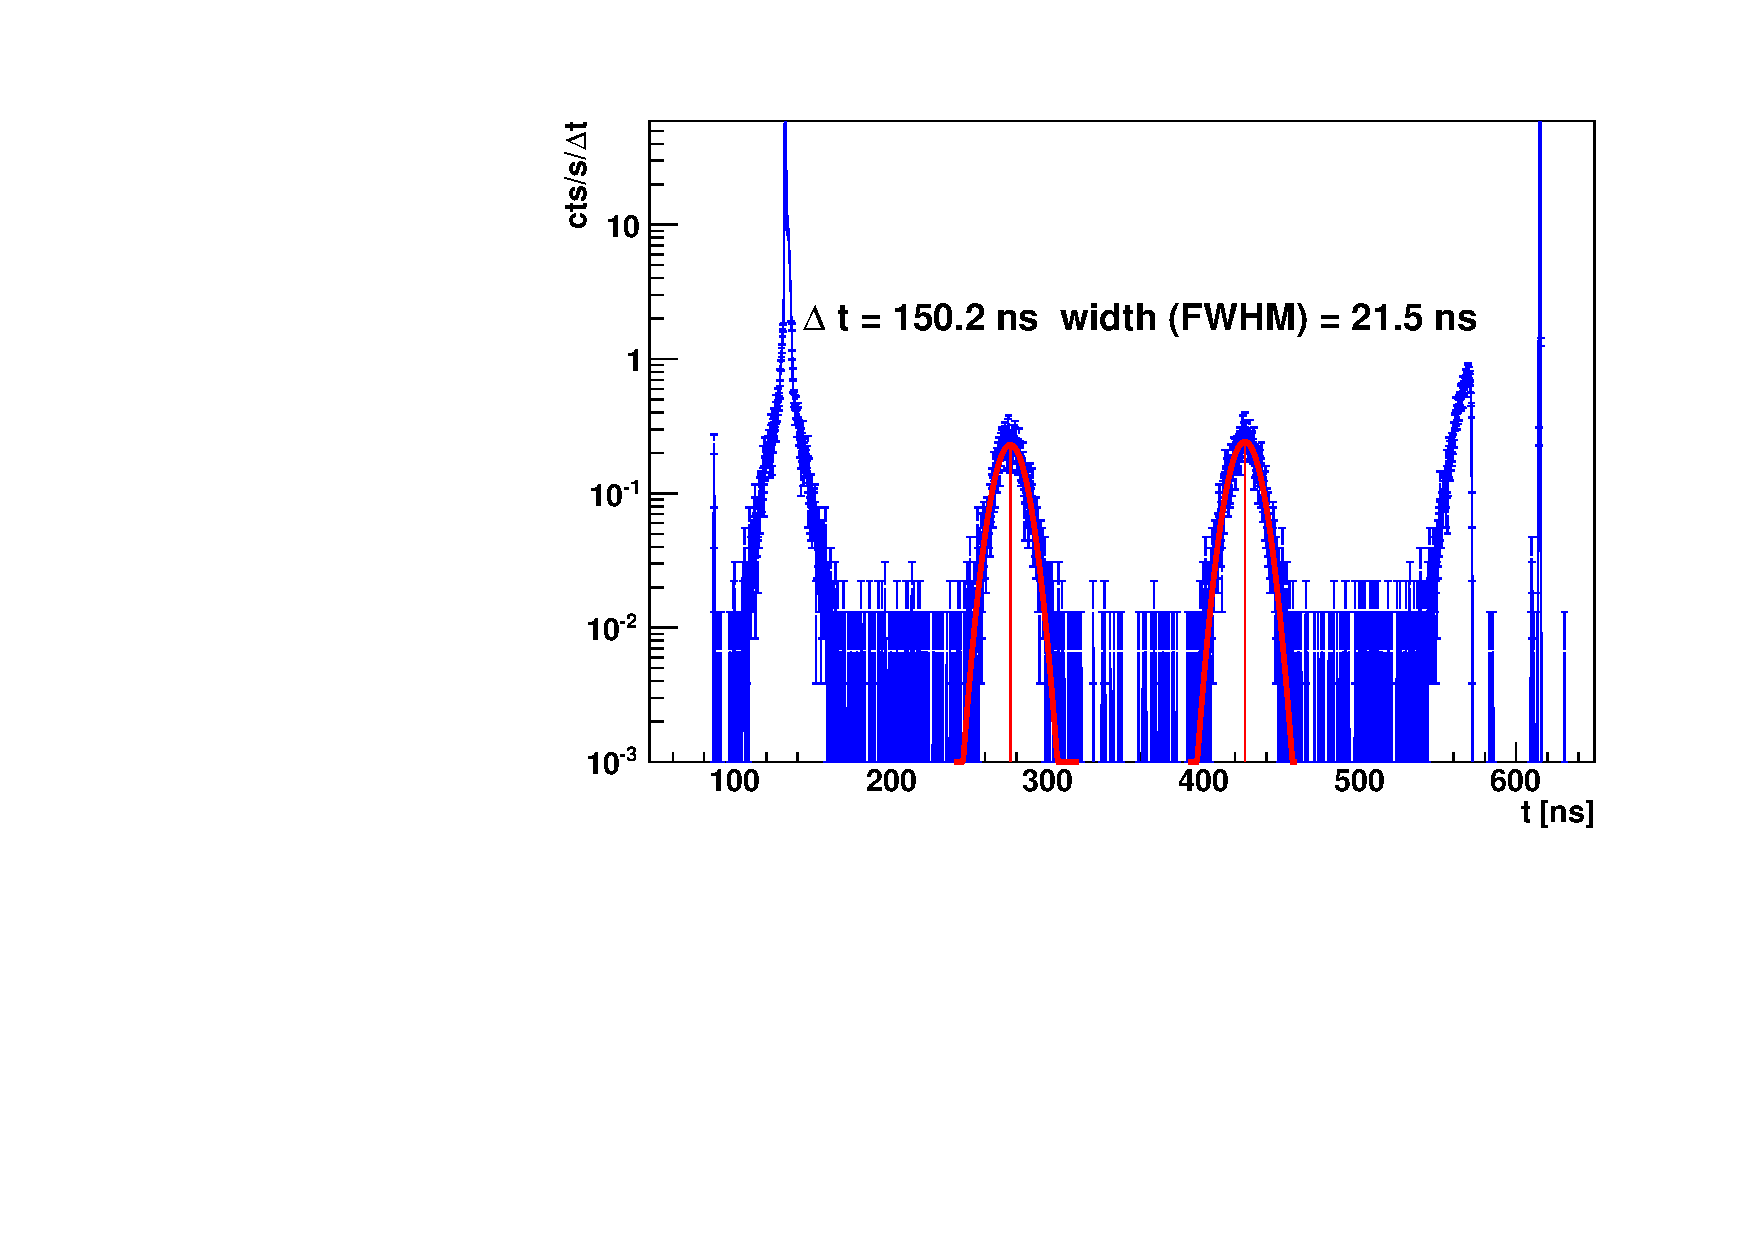
\includegraphics[width=0.6\textwidth]{./Figure/fiber_vert_hor_run14.pdf}
	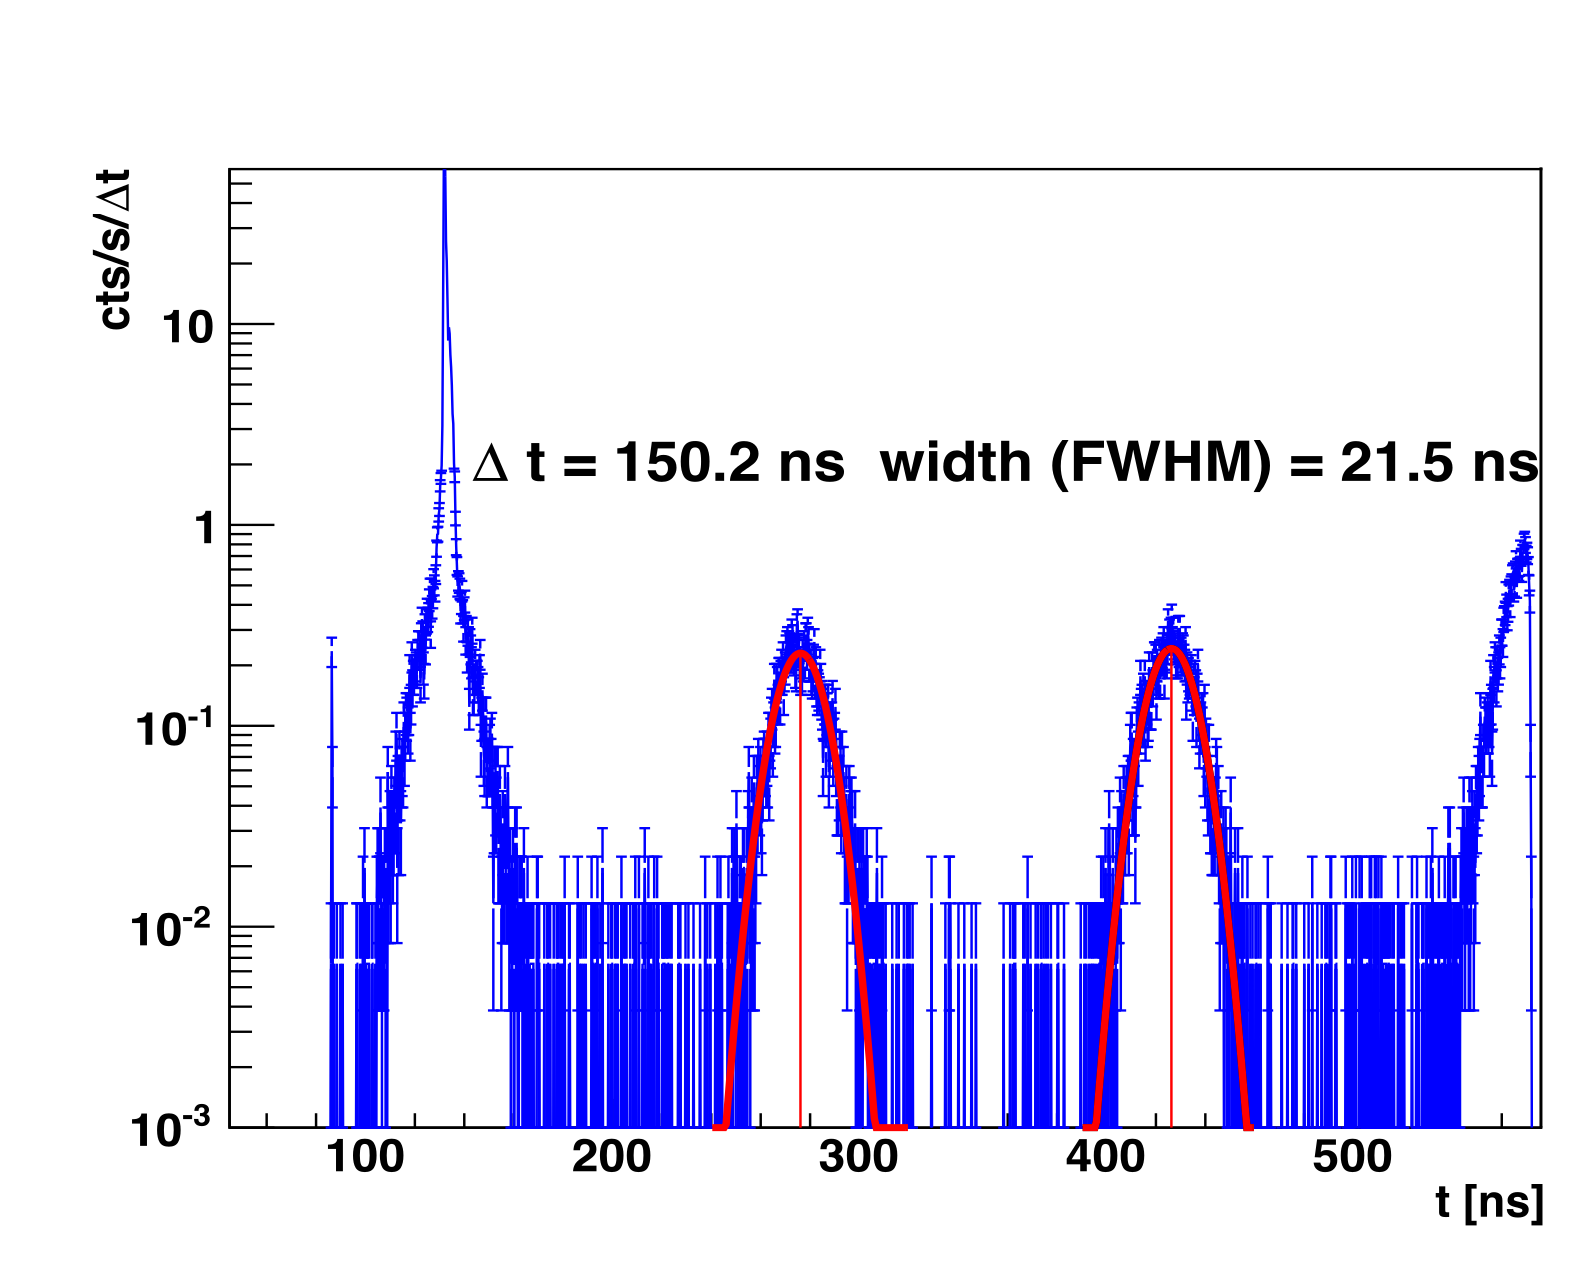
\includegraphics[width=0.6\textwidth]{./Figure/BeamTimeStruct.png} 
  \caption{Beam time micro-structure measured from a carbon ion beam at 400~MeV/u delivered at HIT (time difference between two crossed-scintillating fibers). The offset between the two fibers is arbitrarily set to 130~ns. The pulses have an extraction period of 150.2~ns and the bunches are 21.5~ns FWHM.  On the horizontal axis the time has been measured with a two-scintillating-fiber hodoscope, with 1~ns FWHM time resolution.}
  \label{fig:fig_structure_temps_faisceau_HIT_2013_CC_simulation_Hadronth}
\end{figure}


\subsubsection{Beam modeling}\label{beam_modeling}
The two main beam particles used in clinics are considered in the simulation: protons and carbon ions. The beam range of interest is 15.2~cm in the PMMA phantom, and the associated energy is 160~MeV for protons and 305~MeV/u for carbon ions.\\ 
The beam transverse dimension is modeled with a Gaussian distribution with a standard deviation of 5~mm for protons at 160~MeV and 3.5~mm for carbon ions at 305~MeV/u. The number of incident ions for a spot in pencil beam scanning (PBS) mode is $10^8$ for protons (distal spot - upper intensity limit) and $10^5$ for carbon ions (average spot intensity)~\cite{Kramer:2000aa, Grevillot_2011,smeets_2012}. In the simulation, the beam intensity is modeled by an average number of particles per bunch. The exact number of particles in each bunch is given by a random extraction from a Poisson distribution, where the mean value is the selected beam intensity.\\
The beam time structure is applied at the data analysis stage. Two different time structures have been considered for this study, related to two kinds of accelerators used in clinical practice: the IBA C230 cyclotron for protons (used in 16 clinical centers worldwide) and the HIT synchrotron for carbon ions. For protons at 160 MeV, the primary particles are grouped in bunches of 2~ns (this value may vary also according to the distance between the cyclotron and the treatment room, and energy spread selection) at a frequency of 106~MHz (9.42~ns)~\cite{Roellinghoff_2014}. The clinical beam intensity is 3.2~nA which corresponds to about 200 protons per bunch. Concerning the carbon ion beam at 305~MeV/u, the simulated time structure refers to the measurements presented in section~\ref{beam_measurement}. We used 30~ns duration bunches at a frequency of 5.9~MHz (170~ns period). The clinical beam intensity for carbon ions is $5\times10^7$~ions/s during extraction, corresponding to about 9~ions per bunch. The macro-structure ($~$50\% duty cycle with [1,5]~ns period) is not considered. 

The coincidence window (between scatterer and absorber events) is set to 40~ns, centered on each absorber detected interaction. This value is adapted to the detectors time resolutions. At the simulation stage, each interaction in the detector layers is collected with the related local time. The beam time structure is then applied to each single hit, and the selected coincidence window is used to retrieve scatterer-absorber coincidence events, which are classified as described in section~\ref{MatMeth::events} in various types of true and random coincidences.\\ 
Table~\ref{table:definition_beam_structure_CC_hadrontherapy_Geant4} summarizes the presented beam time structures and coincidence reconstruction features.

\begin{table} [!htbp]
\footnotesize
\centering
\caption{Description of the two beam structures studied: the IBA cyclotron C230 for protons and the synchrotron installed at the Heidelberg Ion Therapy Center (HIT) in Germany for carbon ions. The macro-structure of the synchrotron, at the second time scale, is not considered here. The beam structures are applied to the simulation data.}
\setlength{\tabcolsep}{2pt}
%\hspace{-2.1cm}
\begin{tabular}{c|c|cc}
%\cline{2-4}
\hline
		\multicolumn{2}{c}{ }		 & 					\textbf{Protons} & \textbf{Carbon ions}\\ 
\hline
%\cline{2-4}%\hline
\multirow{3}{*}\textbf{Clinical features}		&	Facility	& IBA Cyclotron C230 &   Synchrotron at HIT\\
											& Clinical intensity& $  2\times10^{10}$ p/s  & $  5\times10^{7}$ ions/s\\
											& Energy 			&160~MeV 			&    305~MeV/u\\
%\cline{2-4}%
\hline
\multirow{3}{*}\textbf{Beam structure}		&	Bunch time [ns]	& 3.2				&  30\\
											& Period [ns]		&   9.4 				& 170\\
											& Primaries/bunch 	&217 			& 9\\
%\cline{2-4}%
\hline
\multirow{2}{*}\textbf{Detectors}						& Coincidence window [ns]		& 40 	&  40 \\
											&Time resolution (FWHM) [ns] & \multicolumn{2}{c}{Si: 15 and BGO: 3}\\
%\cline{2-4}%
\hline
\end{tabular}
\label{table:definition_beam_structure_CC_hadrontherapy_Geant4}
\end{table}



%\newpage
%---------------------------------------------------------------
%---------------------------------------------------------------
\subsection{Compton camera events}
\label{MatMeth::events}

The Compton detection principle is based on the time coincidence of at least one scatterer and one absorber gamma interaction, where an interaction is defined as an energy deposit in a detector module, with the spatial selections detailed in section~\ref{SimuSetup}. As discussed in section~\ref{subsection:modelisation_fasceau_ions_CC_hadrontherapy_Geant4}, the coincidence reconstruction relies on a defined time window, fixed according to the detector resolution. In a simulation environment, different kinds of coincidence events can be distinguished and studied: 
\begin{itemize}
\item[-] real coincidences: created by a single photon first interacting in the scatterer stack and then in the absorber block array;
\item[-] quasi-simultaneous interaction of two secondary particles;
\item[-] double interaction of the same particle, not a photon (e.g. protons, neutrons).
\end{itemize}
As described in section~\ref{SimuSetup}, the simulation setup selects events with absorber interactions limited to a single BGO block.
Concerning the scatterer section, among the real coincidences, three different kinds of events can be identified:
\begin{itemize}
\item[-] single Compton interaction in one silicon layer;
\item[-] multiple gamma interactions in more than one silicon layers;
\item[-] electron escape events.
\end{itemize}
As mentioned in the introduction, events involving more than one photon interaction in the scatterer layers are advantageous since the total absorption of the detected prompt gamma is not required to reconstruct the Compton cone. However, the actual selection of such kind of events with respect to background interactions in real conditions is hardly achievable.

On the other hand, electron escape events can be in principle identified and exploited. They are characterized by two or more scatterer layers involved: if the first Compton interaction in one layer provide enough energy to the recoil electron, it can escape the silicon plane and be detected by one (or more), following planes. Thus, such events can be identified by the electron tracking, and carry additional information with respect to a Compton interaction with no electron escape. The electron tracking allows to reduce the reconstructed Compton cone to a arch of the cone, by the overlap of the cone with the electron tracking plane.      

\subsection{TOF and energy based data selection}
\label{MatMeth::TOF_Ecut}

In an experiment the collected data are affected by a certain number of the so-called random coincidences, which cannot be experimentally distinguished from true coincidences, from the timing coincidence point of view. Such a background level depends on the detector time resolutions, the fixed time coincidence window and the beam time structure, the phantom composition and the camera prototype setup.
In addition to this, the prompt gamma measurement is contaminated by other secondary particles (mainly massive and charged particles like protons and neutrons, but also electrons in the low energy regime), produced by the interaction of the primary particles with the patient/phantom. In figure~\ref{fig:fig_explication_coincidence_CC_simulation_Hadronth}, a schematic view of the different kinds of possible coincidences is presented.

\begin{figure}
  \centering
  %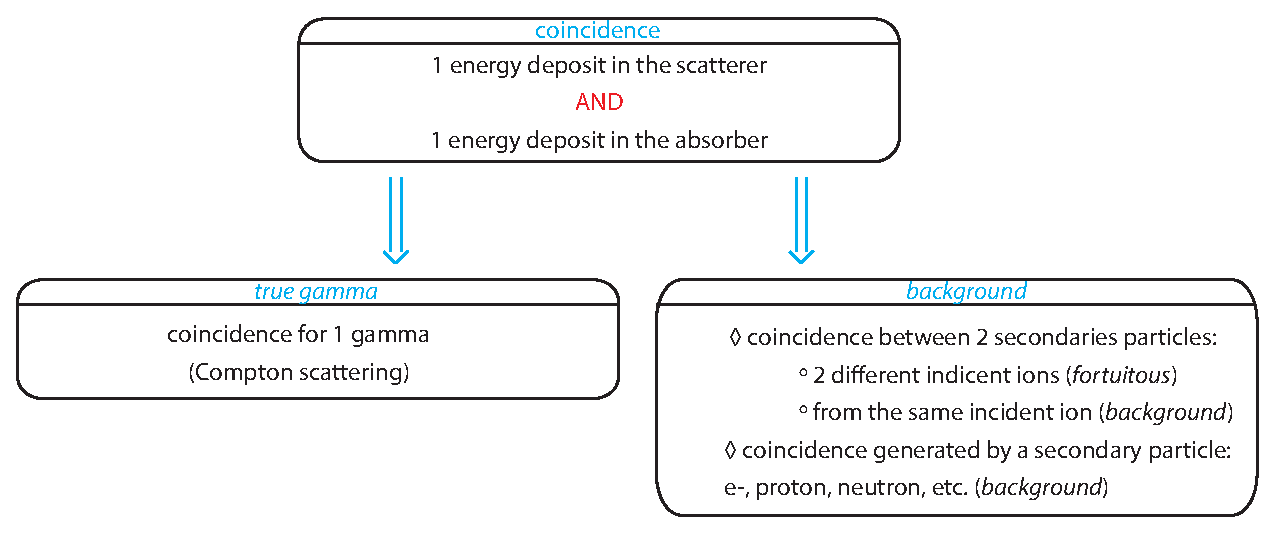
\includegraphics[width=0.9\textwidth]{./Figure/Schema_coincidence_EN.eps}
  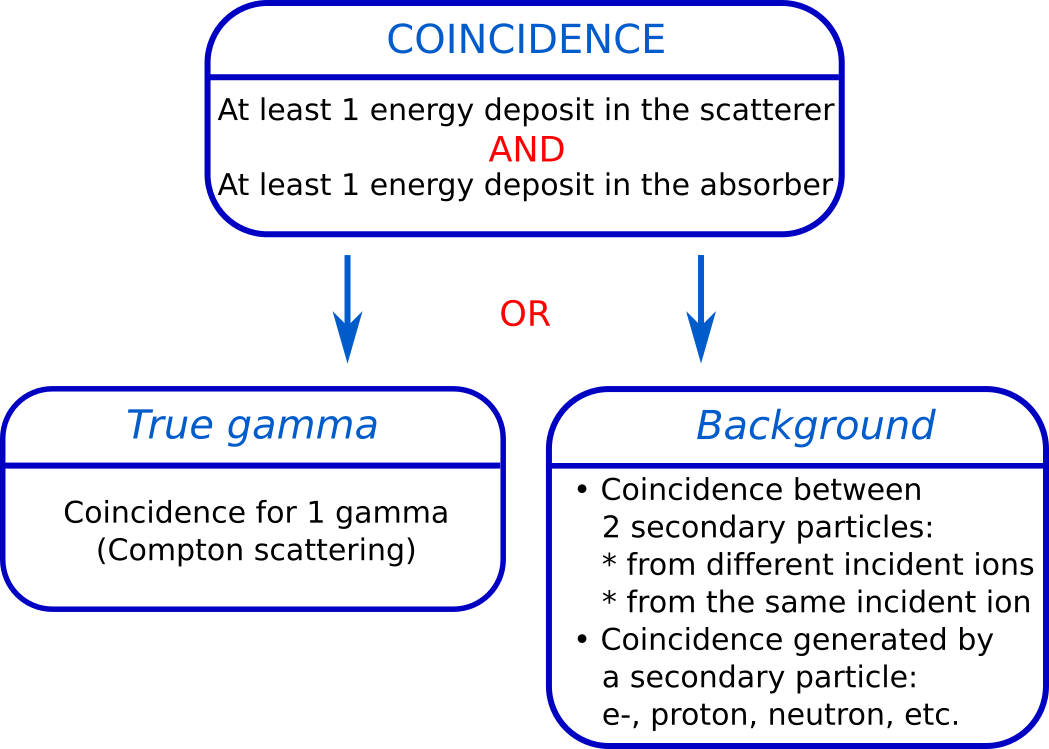
\includegraphics[width=0.7\textwidth]{./Figure/coinc_scheme.png}
  \caption{Diagram showing the different definitions of coincidences in the Compton camera. The energy deposits are selected in the silicon scatterer to be limited to neighboring strips (3 strips maximum), and in the absorber blocks the events are selected to be limited to a single block.}
  \label{fig:fig_explication_coincidence_CC_simulation_Hadronth}
\end{figure}
Ad-hoc filtering methods are applied to reduce the above described contamination.

\begin{itemize}
\item Time-Of-Flight (TOF): it has been demonstrated that a time-of-flight discrimination is possible and effective in reducing the background generated by massive particles interactions~\cite{Testa:2010aa}. The massive particles approach the detector at a lower speed with respect to photons. The time information provided by the hodoscope and the absorber can be combined to fix a detection time window and reject all the events outside the window. The time elapsed between the incident particle detection in the hodoscope and the secondary particle detection in the absorber is considered as the time-of-flight. In order to define the appropriate time window, the TOF spectra of the collected events resulting from the irradiation of the PMMA target with 10$^{8}$ 160~MeV protons have been produced for true gamma coincidences and background events, taking into account the detector resolutions. The result is shown in figure~\ref{fig:fig_TOF_distribution_CC_simulation_Hadronth}. For this study, no time structure have been applied to the primary protons, thus only independent events have been considered. The time-of-flight spectrum resulting from the simulation shows that:
\begin{itemize}
\item the coincidences of interest (produced by prompt-gamma rays) are included in a window between 0 and 8~ns;
\item in the TOF window a comparable amount of true coincidences and background events is observed. Since we consider only independent events, this means that such background events are due to random coincidences between two prompt gammas directly or indirectly induced by the same incident ion. The background events outside the TOF window are due to massive particle interactions in the camera.
\end{itemize}
It is worth to stress that the simulation results shown in figure~\ref{fig:fig_TOF_distribution_CC_simulation_Hadronth} do not include random coincidences, created by prompt photons emitted by different primary ion interactions, and room background, mainly due to neutrons. Both components contribute to the background spectrum. In the case of the C230 cyclotron accelerator, the room background has been measured and showed a flat ditribution in time~\cite{Pinto2014}.

When the beam time structure is applied to the simulated data (including the detector time resolutions), the lists of time-ordered interactions in hodoscope and absorber are produced. For each coincidence events, we look for the first hodoscope event in the 8~ns time window preceding the absorber interaction time. All events with no hodoscope coincidence in the time window are rejected.

\begin{figure}	
  \centering
  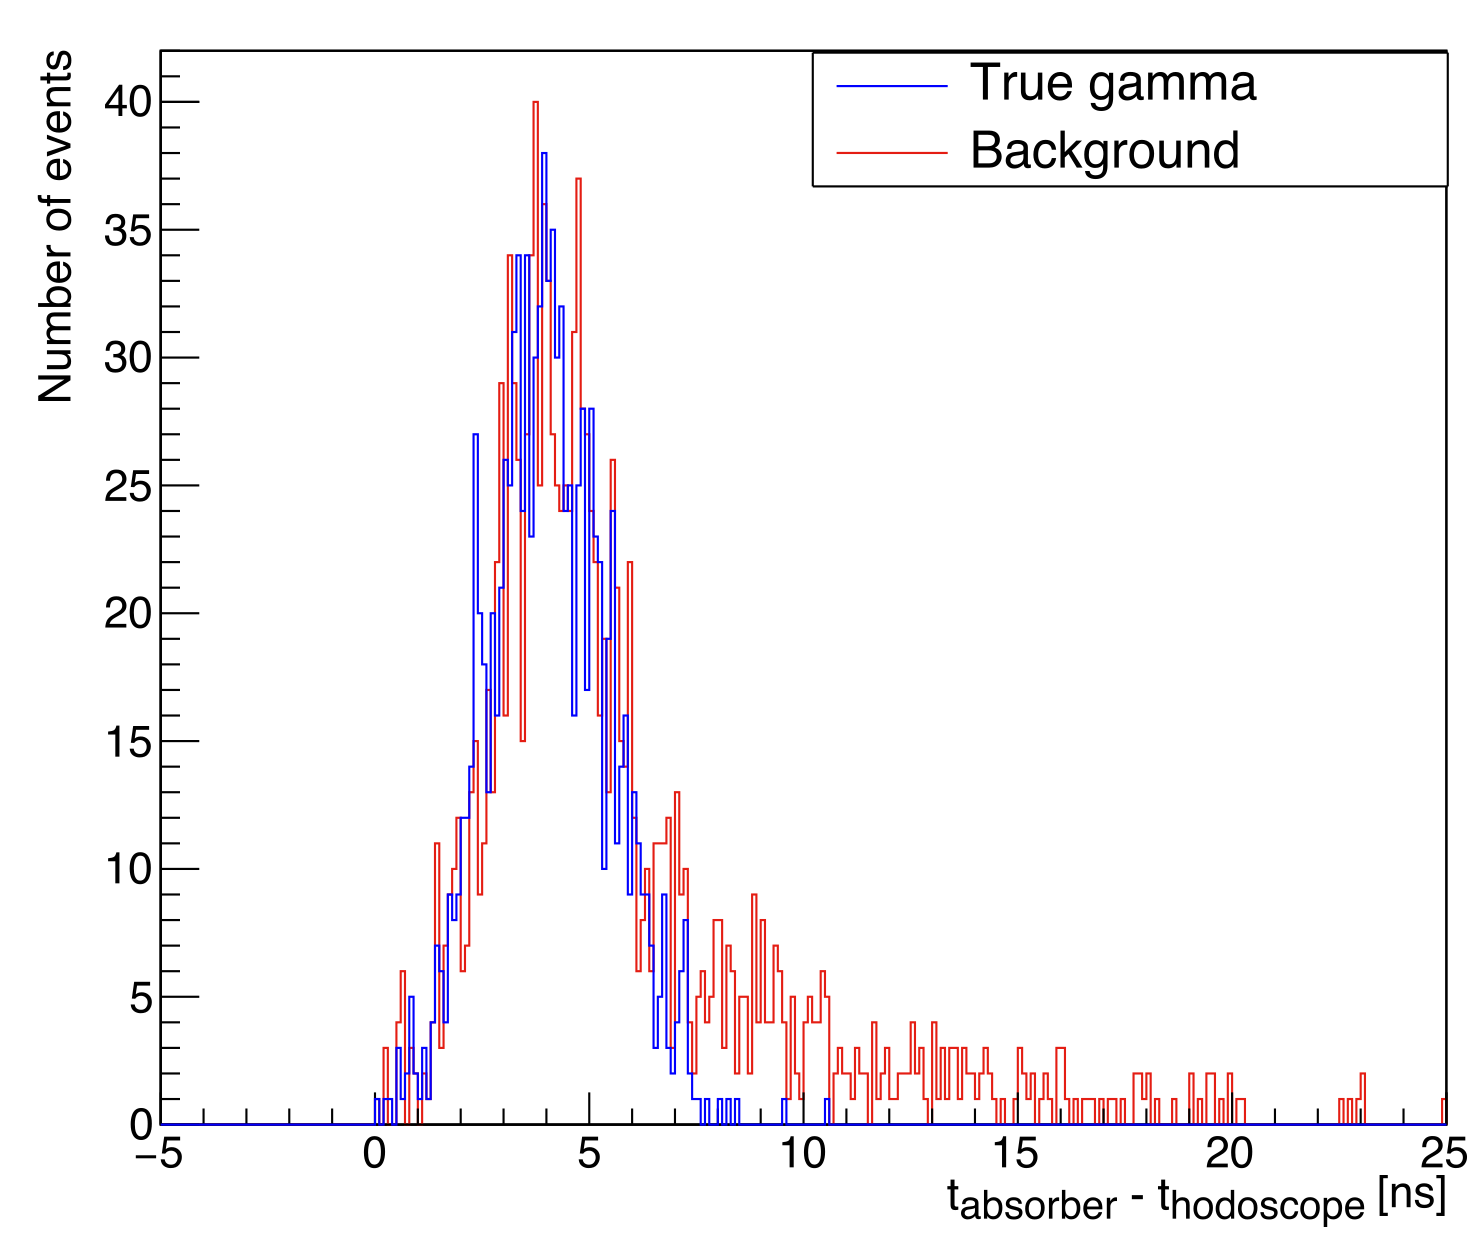
\includegraphics[width=0.6\textwidth]{./Figure/TOFspectrum.png}
  \caption{Time of flight spectra of true gamma coincidences (blue) and background events (red) obtained with $10^{8}$ 160~MeV independent incident protons.}	
  \label{fig:fig_TOF_distribution_CC_simulation_Hadronth}
\end{figure}

\item Energy selection: energy thresholds are defined for the event detection. 50~keV and 100~keV are set as lower threshold for the energy deposited in a single silicon layer and BGO block, respectively. For a complete event, a total absorbed energy lower limit is set to 1~MeV. In addition to the effect of background rejection, this selection also reduces the impact of partially absorbed photons.

Further energy selections, assuming for instance $E_1+E_2$ equal to one of the strong gamma lines, have been applied by other authors~\cite{Draeger:2017aa}. Also, filters checking the possibility of reconstructing a Compton cone could be used. At this stage we did not consider such approaches in order to cope with simple considerations on signal to noise on raw data.

\end{itemize}

\subsection{Reconstruction algorithms}
\label{MatMeth:reconstruction}
Once the coincidences are defined and selected according to the fixed physical cuts, the prompt-gamma emission point has to be reconstructed for each event. This can be done via analytic or iterative algorithms based on the Compton kinematics. Both are presented in the following sections.


\subsubsection{Line-cone algorithm}
The reconstruction via line-cone algorithm exploits the energy deposit and position information collected by the camera in addition to the beam spatial information provided by the hodoscope. Thanks to the deposited energies in the detectors and the interaction positions, a cone surface is analytically defined via the Compton equation~\ref{Compton_equation}. Figure~\ref{fig:reconstruction_scheme} shows a sketch of the reconstruction principle. The interaction position in the scatter gives the cone apex and the line connecting the interaction positions in scatterer and absorber gives the cone axis. We assume that the initial energy of the gamma ray is fully absorbed in the absorber. This assumption has been investigated and the results are shown in section~\ref{Results::efficiency}. In order to constrain the reconstruction, the beam direction is used to limit the possible solutions (lying on the reconstructed cone surface) to two points (intersection of the beam direction and the reconstructed cone). At this stage we do not consider the lateral beam spread in the target, due to multiple scattering. The set of all the reconstructed points gives the emission source distribution. The final image is the mono-dimensional projection of the prompt gamma emission profile. 

\begin{figure}
\centering
  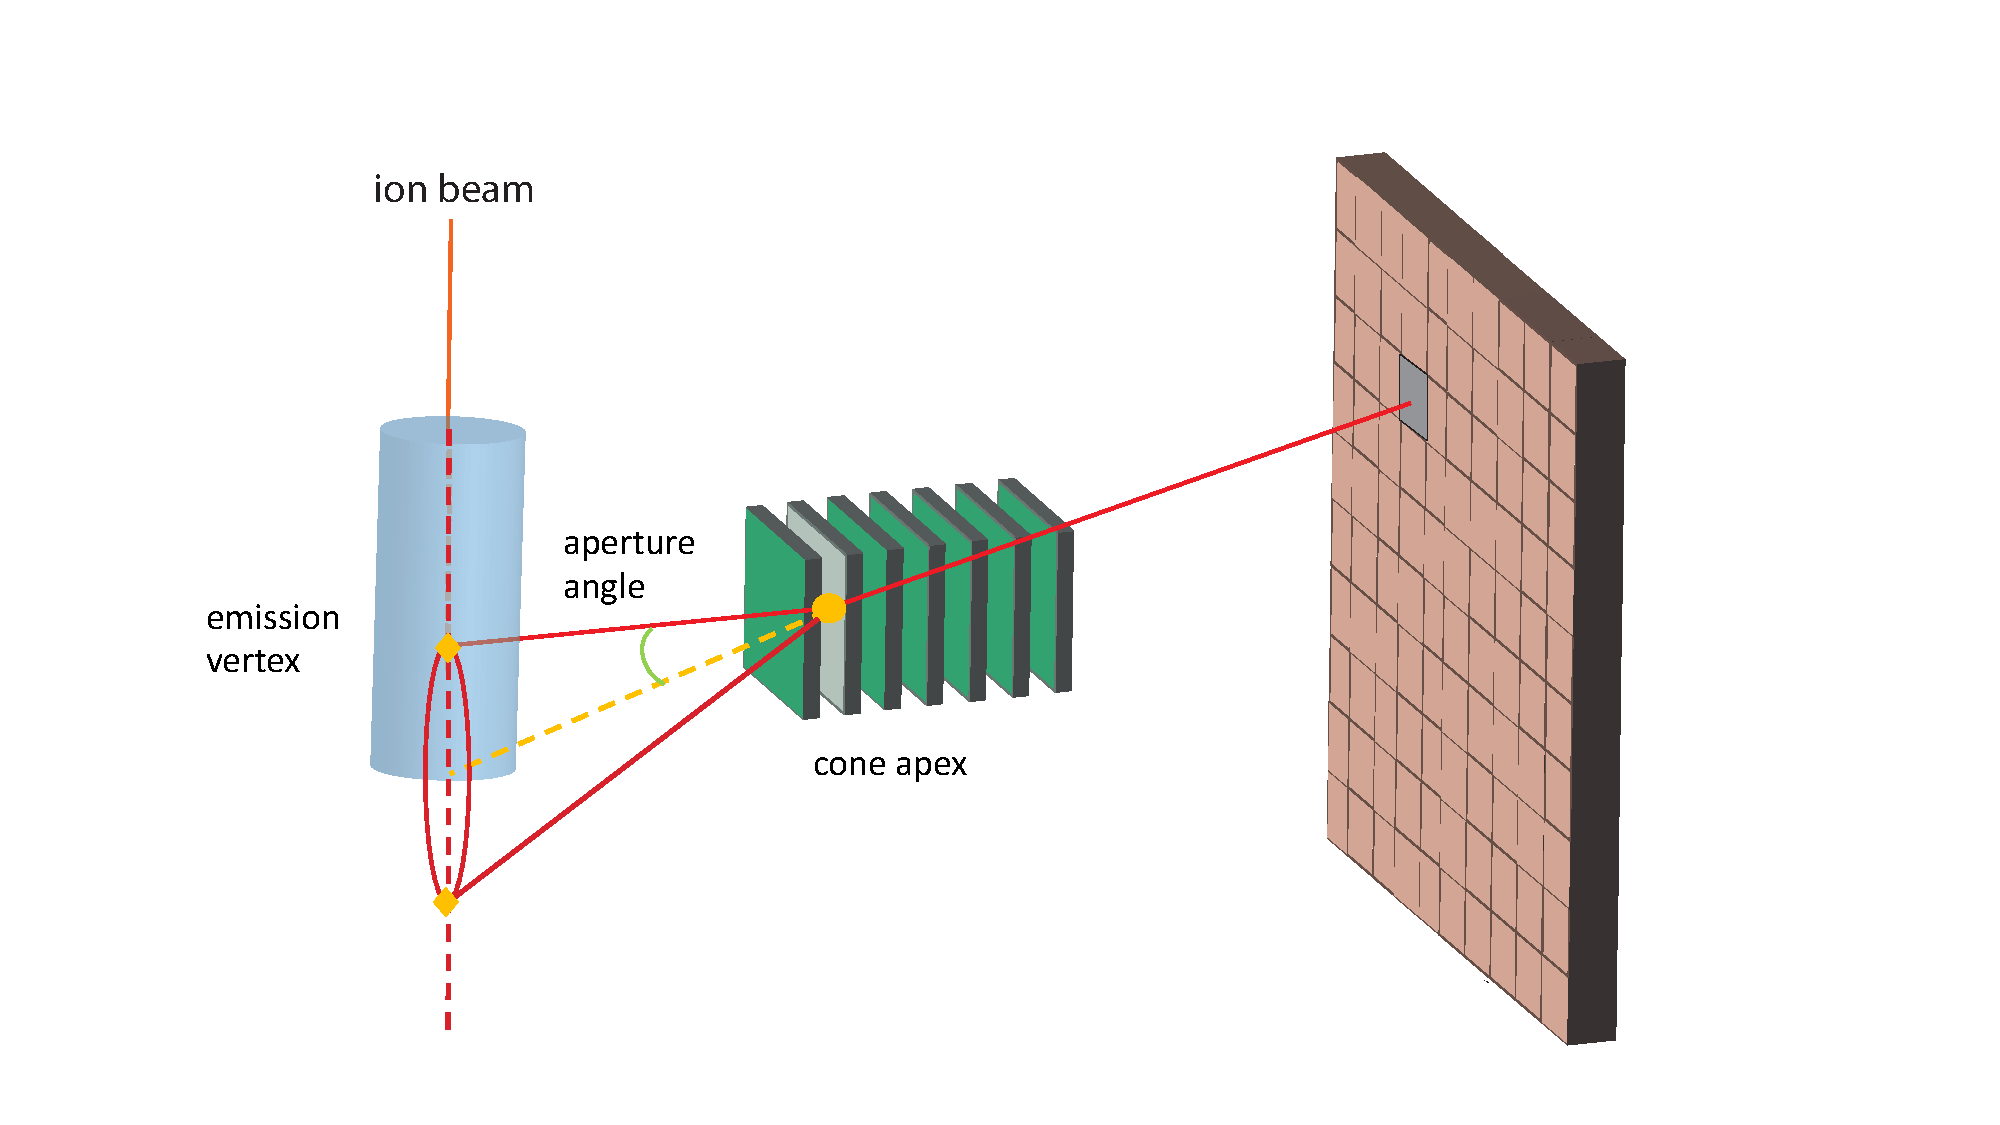
\includegraphics[width=0.8\textwidth]{./Figure/reconstruction_scheme}
  \caption{Scheme of the reconstruction principle for Compton events. For line-cone reconstruction methods, two points are extracted for each event (diamonds in the figure), provided by the intersection between the reconstructed Compton cone and the beam line. The reconstructed image is strictly 1D. For the iterative MLEM algorithm, each algorithm iteration adds constraints to the reconstructed cone surfaces, leading to  a 3D image.}	
  \label{fig:reconstruction_scheme}
\end{figure}

\subsubsection{LM-MLEM algorithm}	
The iterative methods allow to get a 3D image reconstruction, potentially by taking into account the spatial resolution and the energy resolution of the detectors. Several iterative algorithms have been developed for Compton event reconstruction~\cite{schone_common_2010, zoglauer_design_2011,gillam_compton_2011,mackin_evaluation_2012,lojacono_low_2013, Huang2018, Taya2017, Schoene2017}.

The \textit{List-Mode Maximum Likelihood Expectation Maximization} (LM-MLEM) algorithm is a MLEM version which enables one to reconstruct the image directly from the list of detected events.
The features of the LM-MLEM algorithm used for this study are detailed in~\cite{hilaire_compton_2014}.%\cite{maxim_filtered_2014,hilaire_compton_2014}.%\cite{maxim_analytical_2009,lojacono_low_2013,maxim_filtered_2014,hilaire_compton_2014}.\newline

%The first step is to define the volume which includes the origin of the prompt gamma ray detected. This volume is divided into equal voxels and the emission intensity is assumed homogeneous for each voxel $j$, with a Poisson distribution of parameter $\lambda_j$ (a vector of the emissions intensities of all the voxels). The algorithm is based on a system matrix $T$ composed of the coefficients  $t_{ij}$ which represent the probability that a photon produced in the voxel $j$ is detected in coincidence by the Compton camera as an event $i$. The probability for a gamma detected in coincidence to be emitted from the voxel $j$ is denoted as $s_j$.
%The LM-MLEM algorithm starts with an initial value $\lambda^{(0)}_j$, which can be the simple back-projection reconstruction.
%The iterations rely on the following recurrence relation:
%
%\begin{equation}
%\lambda_j^{(l+1)} =  \frac{\lambda_j^{(l)} }{s_j} \sum\limits_{i=1}^{N_{\gamma}} t_{ij} \frac{1}{P_i^{(l)}},\quad \rm{with}\quad  P_i^{(l)}=\sum\limits_{k=1}^{N_{v}} t_{ij}\lambda_k^{(l)},
% \label{eq:equation_lambda_compton_med_nucleaire}
%\end{equation}
%where $N_{\gamma}$ is the number of detected events and $N_v$ is the number of voxels in the image.
%
%For each photon detected, the coefficients in column i are calculated by taking into account the uncertainties on the angle between the source and the involved scatterer plane and the angle between the scatterer plane and the absorber involved module.
%The matrix elements $t_{ij}$ are calculated as:
%\begin{equation}
% t_{ij} = K(\beta_i,E_{tot})\frac{|\rm{cos}(\theta_{{V_2V_1}}) |}{V_2V_1^2} \int\limits_{M\in v_j} \frac{|\rm{cos}(\theta_{V_1M})|}{V_1M^2} h_i(M)dv,
% \label{eq:equation_tij_compton_med_nucleaire}
%\end{equation}
%where $\beta_i$ is the Compton scattering angle, $V_1$ the interaction position in the scatterer, $V_2$ the interaction position in the absorber, $h_i$ the spatial kernel which models the uncertainties on the Compton angle for each voxel $M$, $K(\beta_i,E_{tot})$ the differential cross section and $v_j$ the reconstructed volume.
%
%In order to simplify and speed up the calculation of the $t_{ij}$ matrix, the voxels located far from the reconstructed cone are set to 0. The distance between the cone and the voxel is calculated by taking the voxel center as reference point. %The spatial resolutions are not included in this version of the algorithm.\newline
%For each iteration, the matrix $T$ is stored and the reconstructed image can be produced.


\subsection{Performance study}
\label{MatMeth:performance}
In this section the parameters studied for the camera performance evaluation are explained. The study is mainly divided into four sections:
\begin{itemize}
\item Detection efficiency of various types of true coincidences: the camera efficiency for the detection of the various kinds of true coincidences defined in section~\ref{MatMeth::events} is studied by means of mono-energetic irradiation with point-like sources as a function of the incident gamma energy;
\item Absolute efficiency: the camera absolute efficiency for the detection of events with a single scatterer layer involved is studied by means of mono-energetic irradiation with point-like sources as a function of the incident gamma energy and the source position with respect to the camera;
\item Rate of background coincidences: with proton and carbon beams interacting with the PMMA phantom, the rate of background and true detected coincidences (for events with a single scatterer layer involved) is studied as a function of the beam intensity;
\item Camera precision: the camera capability of identifying the fall-off of the prompt-gamma emission profile is tested and the two reconstruction methods presented above are compared (for events with a single scatterer layer involved). 
\end{itemize}

\subsubsection{Detection efficiency of various types of true coincidences}\label{relEff}
The efficiency is crucial for the Compton camera performances and for its possible application in treatment monitoring. An efficient monitoring system should be ideally in real time, in order to allow for a treatment adaptation or interruption in case of severe issues detected in the delivered dose profile with respect to the planned treatment. In order to achieve an online detection of such deviations, given the limited prompt gamma emission rate per incident ion~\cite{Ortega:2015aa}, a high detection efficiency is required to perform a monitoring on, ideally, a beam spot basis. In addition to this, the absolute detection efficiency directly affects the image reconstruction quality, which is in general increased for increased statistics.

The efficiency in the detection of specific kinds of events detailed in section~\ref{MatMeth::events} has been studied with the irradiation from point-like mono-energetic gamma sources. The setup is the same as figure~\ref{fig:fig_setup_CC_simulation_Hadronth}, with the exception of the PMMA phantom which is removed to leave the gamma source in air. Different energies have been tested to mimic different prompt gamma lines: 300~keV, 500~keV, 1~MeV, 2~MeV, 4~MeV, 6~MeV. No time structure is reproduced for this part of the study.
In addition, the rate of events with an almost full primary energy absorption has been studied for the various kinds of coincidences as a function of the primary gamma energy. The threshold for the energy absorption has been set to 90\% of the primary gamma energy. 
The results of this preliminary study (see section~\ref{Results::efficiency}) determined the choice to limit the next investigations to events with a single scatterer plane involved; all events with more than one scatterer layer hit have been rejected for the analysis described from section~\ref{absEff} and the results presented from section~\ref{Results::efficiency}.

\subsubsection{Absolute detection efficiency}\label{absEff}

The absolute efficiency $\epsilon$ for the detection of coincidences with a single scatterer plane hit is defined as:
\begin{equation}
\epsilon =\frac{\mathrm{N}\gamma_{\mathrm{coinc}}}{\mathrm{N}\gamma_{\mathrm{total}}},
\end{equation}
\label{eq:equation_efficacite_absolue}
with $N\gamma_{\mathrm{coinc}}$ the number of gamma events corresponding to the selected true coincidences , $N\gamma_{\mathrm{total}}$ the total number of emitted gammas.
In addition to its dependence on the gamma energy in the range 300~keV - 6~MeV (see section~\ref{relEff}), the absolute efficiency has been also studied as a function of the point-like source position. The source is set in the range $-300$~mm to $+300$~mm (with the center of the camera transverse section set in the position 0), and moved with variable length steps, up to 1~cm. The movement followed the transverse axis of the camera. 

\subsubsection{Rate of background coincidences}

As the Compton detection principle relies on time coincidences, in addition to the main importance played by the detectors energy resolutions, the beam intensity and time structure are important parameters to be studied in order to assess the possible clinical implementation of a Compton detection based monitoring of ion beam treatment. The ability of the detection system to distinguish between true and background coincidences, i.e.~the resulting signal over noise ratio, strongly depends on the beam time structure. The number of true and background coincidences is studied as a function of the beam intensity, before and after data reconstruction via line-cone algorithm~(see section~\ref{MatMeth:reconstruction}). To be noticed that, following the results of the efficiency study (see section~\ref{Results::efficiency}), only events with one single scatterer layer hit are selected. 

The range of intensities is defined in order to cover a wide range of operation: from a very low beam intensity to a realistic clinical particle rate. Therefore, for proton and carbon ions, the lowest beam intensity is set to 0.1 particles per bunch on average, while the upper limit is set to 217 protons or 70 carbon ions per bunch. All the simulations are performed with a total of $10^{8}$ primary protons and  $2\times10^{5}$ primary carbon ions (see section~\ref{beam_modeling}). For the analysis of the results, the coincidence yields are scaled to the number of incident ions.

\subsubsection{Camera precision}
\label{MatMeth:precision}

The camera precision is defined as the difference between the predicted PG fall-off position - FOP - (according to the treatment planning) and the detected one.
In this study, a reference profile has been defined as the reconstructed emission vertex profile at high statistics ($\mathrm{10^{10}}$ incident protons). This FOP is used as reference and compared to the ones at lower statistics, deduced as described in the following.

For the LM-MLEM reconstruction, the reconstruction volume is set to $20\times40\times1$~cm$^3$ around the expected FOP, with a $101\times201\times5$ voxel matrix. To be noticed that the two reconstruction methods produce different results: the line-cone method is based on the beam direction information, so that it naturally returns a mono-dimensional image as result, while the LM-MLEM method is able to reconstruct the prompt-gamma emission distribution in three dimensions. A mono-dimensional projection along the beam direction is used for the fall-off identification and for a direct comparison of the line-cone method.
The \textit{SmoothKern} method, with the Nadaraya-Watson regression~\cite{Nadaraya_regression, Watson_regression}, is used to smooth the reference profiles in order to reduce relative statistical fluctuations.

A region of interest (ROI) ranging from $y=0$ mm to $y=+100$ mm is defined around the expected FOP, located at $y=+50$~mm in the phantom. The reference reconstructed profiles are modeled in the ROI by a linear combination of Non-Uniform Rational Basis Splines (NURBS)~\cite{NURBS}. 

The reference data set is normalized in order to obtain lower statistics profiles, in the range 1$\times$10$^8$ to 5$\times$10$^9$. Statistical fluctuations, randomly extracted following a Poisson law, are added to the obtained PG profiles to mimic realistic reconstructed profiles. This method is used to reduce the analysis time.

For each chosen statistics, 1000 PG profiles are generated and a custom minimization method is applied to deduce the minimal shift between the reference profile and the one at lower statistics. The minimization algorithm shifts the reference profile in a 60~mm range, between $-30$~mm and $+30$~mm with respect to the initial position, with a step of $0.1$~mm, and for each position it compares its position to the low statistics profile by calculating the $\chi^2$ as follows:
\begin{eqnarray}
\chi^2 = \sum\limits_{i=1}^{N_{bin}} {(y_{\mathrm{sample,i}}-y_{\mathrm{NURBS,i}})^2},
\end{eqnarray}
where for every bin $i$ $y_{\mathrm{sample}}$ is the number of events in the low statistics profile, $y_{\mathrm{NURBS}}$ is the number of events for the reference profile NURBS (scaled at the same low statistic). 
%Several minimization algorithms are available, but in order to avoid artifacts at low statistic, the following robust approach has been preferred.
The described approach is robust and allows to avoid artifacts at low statistics.
%Figures~\ref{fig:fig_Results_Chi2_Distribution_Variation_CC_simulation_Hadronth_LC} and~\ref{fig:fig_Results_Chi2_Distribution_Variation_CC_simulation_Hadronth_MLEM} show the distribution of $\chi^2$ calculated for a low statistic profile at $10^8$ incident protons.

The global minimum of all the calculated $\chi^2$ is then retrieved and the shift associated to this value is added to the shift distributions. % shown in figure~\ref{fig:fig_Results_Precision_Distribution_Variation_CC_simulation_Hadronth_LC} and~\ref{fig:fig_Results_Precision_Distribution_Variation_CC_simulation_Hadronth_MLEM} for the line-cone and LM-MLEM algorithm respectively, for $10^8$ incident protons. 
The standard deviation of the distribution resulting of the thousand results gives the precision of the camera for a given number of incident protons. 



% \begin{figure}
% \centering
% \subfloat[\label{fig:fig_Results_Estimation_Camera_Profil_highStat_CC_simulation_Hadronth_LineCone}]{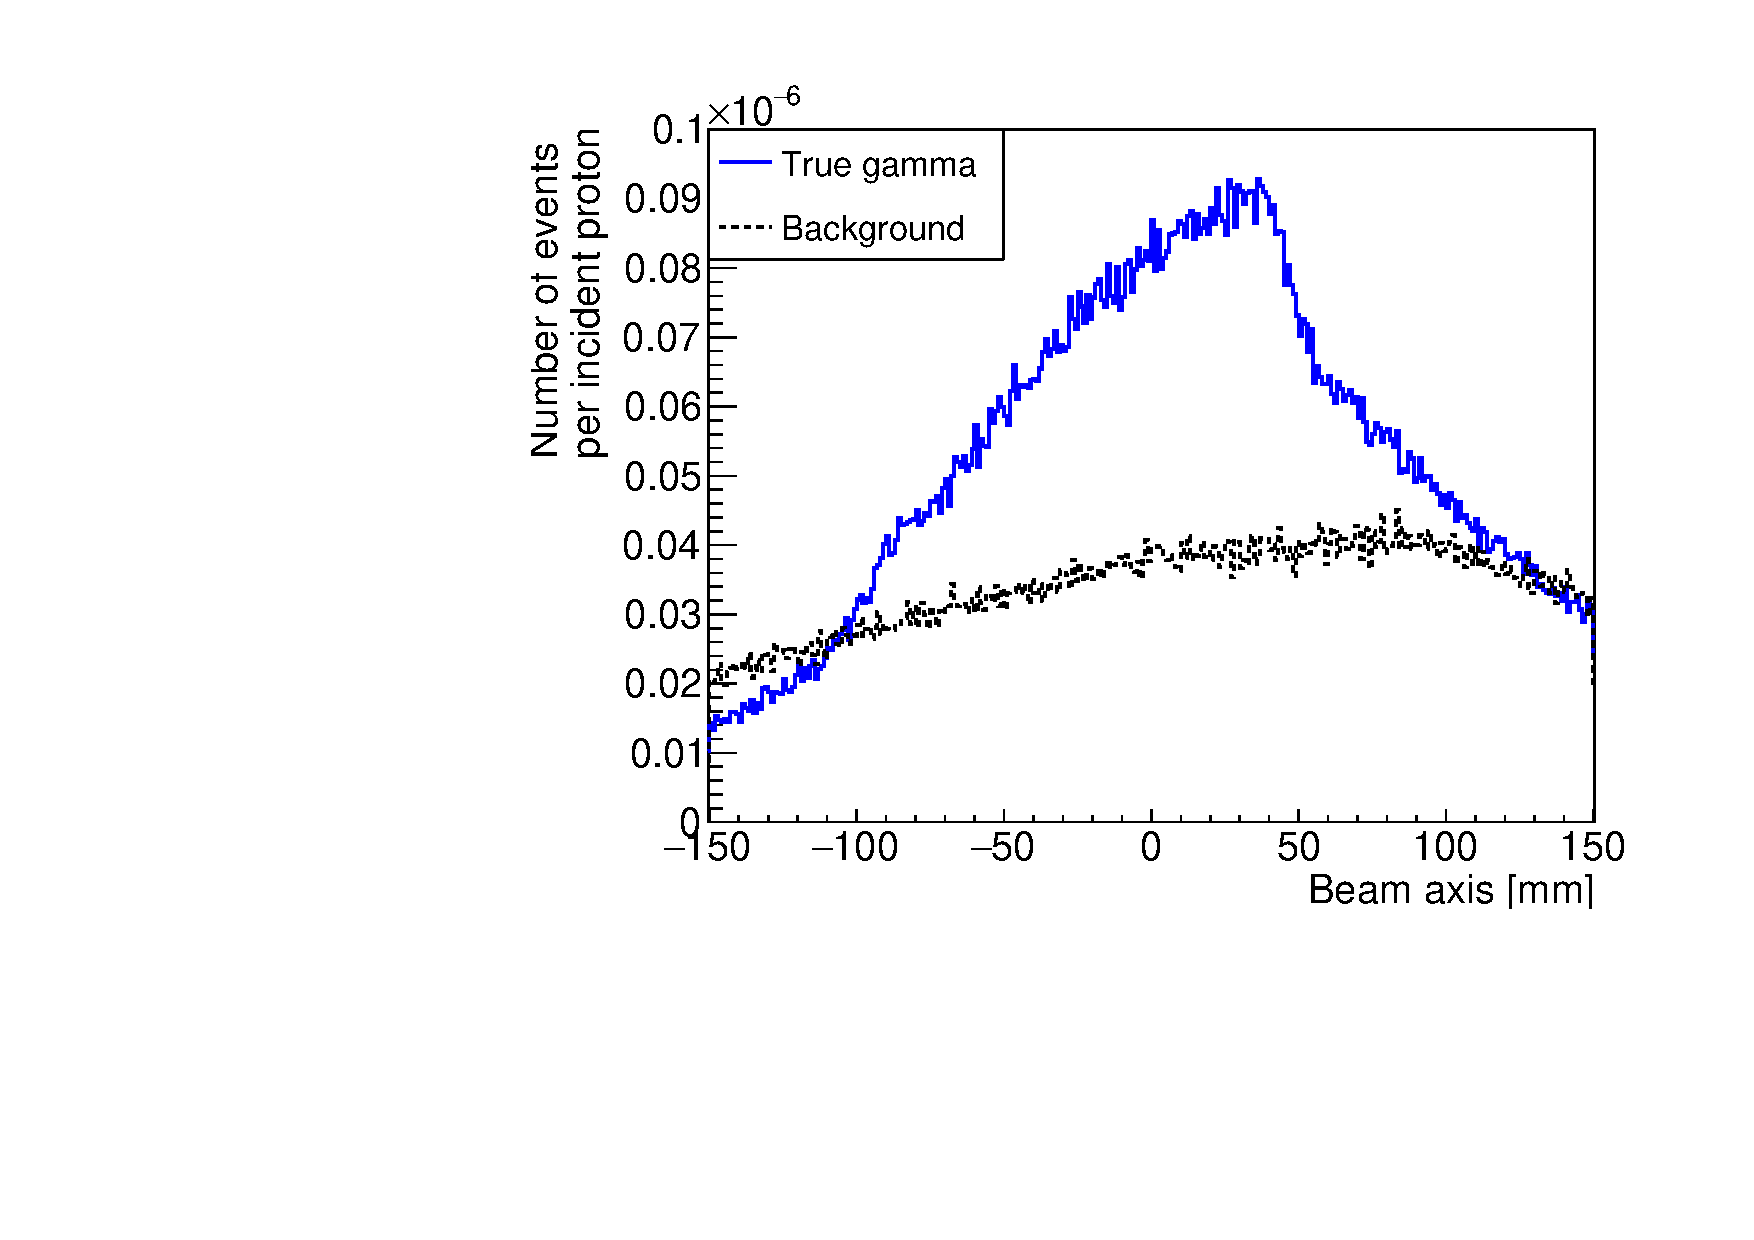
\includegraphics[width=0.33\textwidth]{./Figure/profile_high_stat_linecone_2.pdf}}
% \subfloat[\label{fig:fig_Results_Estimation_Camera_Profil_highStat_CC_simulation_Hadronth_MLEM}]{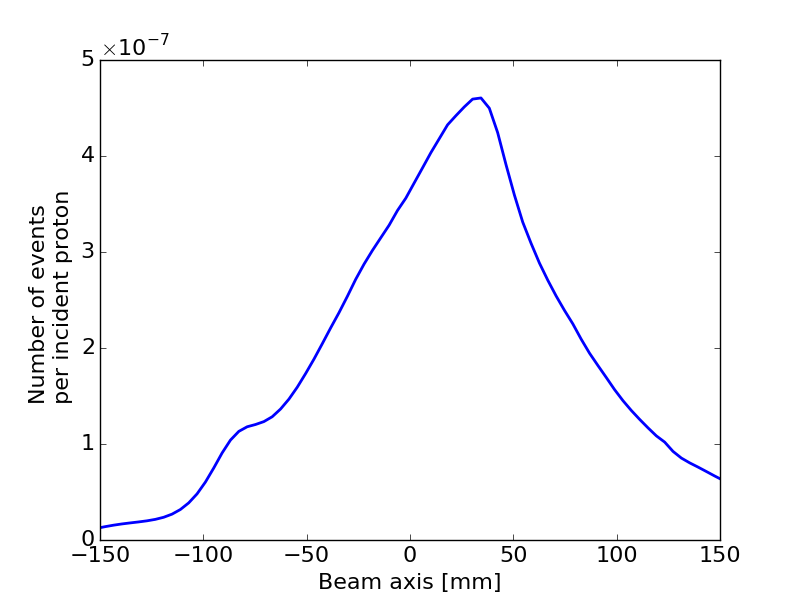
\includegraphics[width=0.32\textwidth]{./Figure/profileY_corr_r15.png}}\\
%  %\subfloat[\label{fig:fig_Estimation_Camera_CC_NURBS_Poisson_LC}]{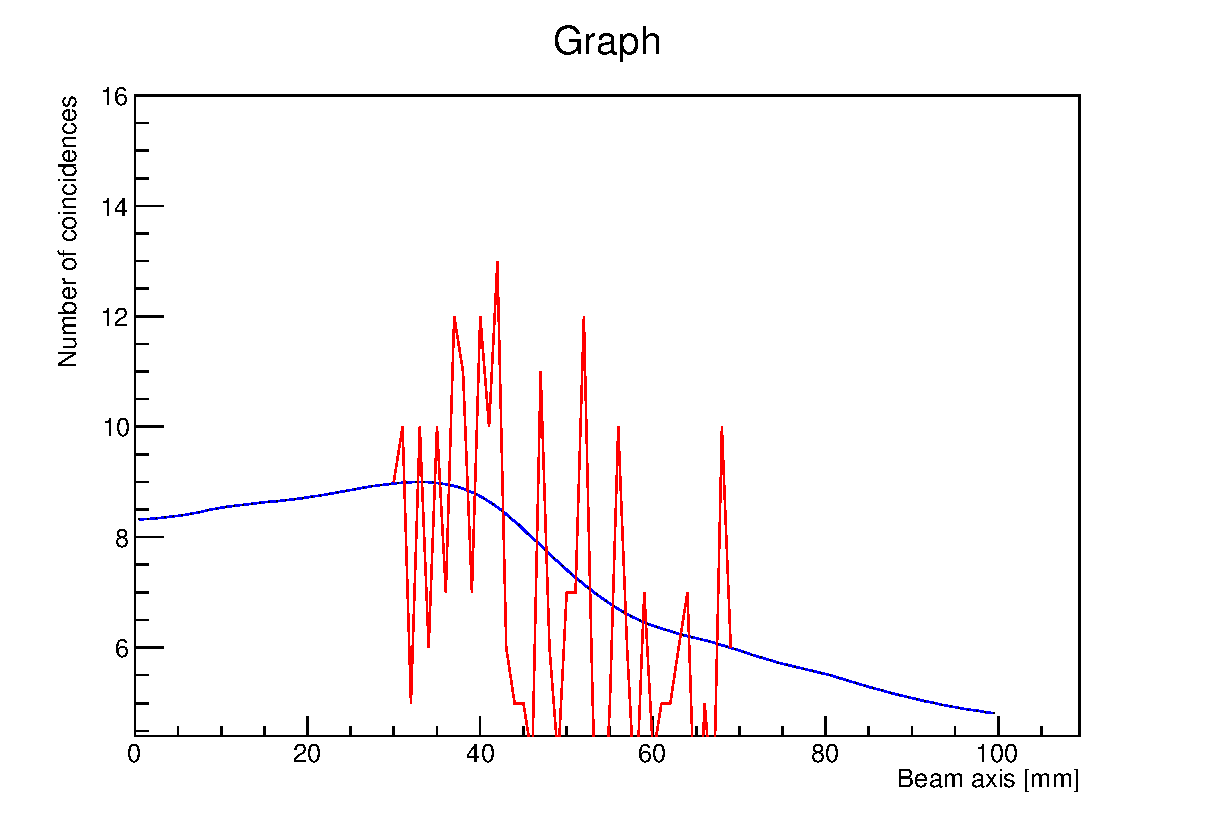
\includegraphics[width=0.33\textwidth]{./Figure/2017-08-02_Poisson_Nurbs_1e8_Article_LC.eps}}
%  \subfloat[\label{fig:fig_Estimation_Camera_CC_NURBS_Poisson_LC}]{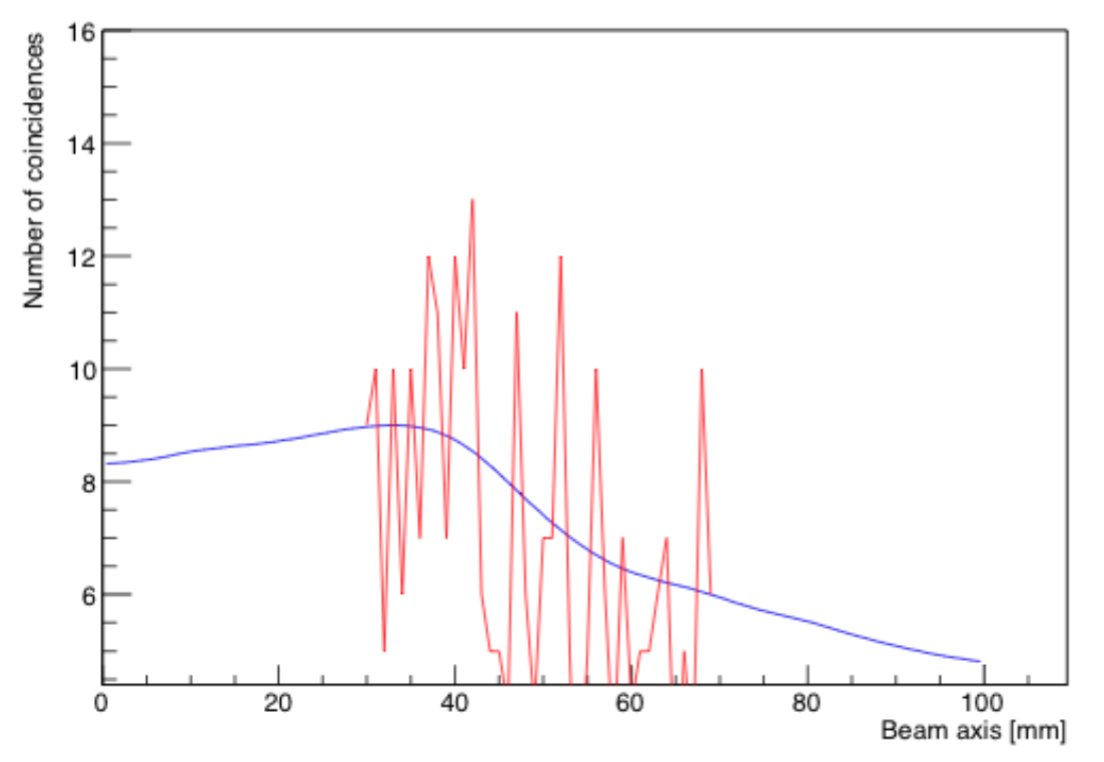
\includegraphics[width=0.33\textwidth]{./Figure/line_cone_NURBS.png}}
%  %\subfloat[\label{fig:fig_Estimation_Camera_CC_NURBS_Poisson_MLEM}]{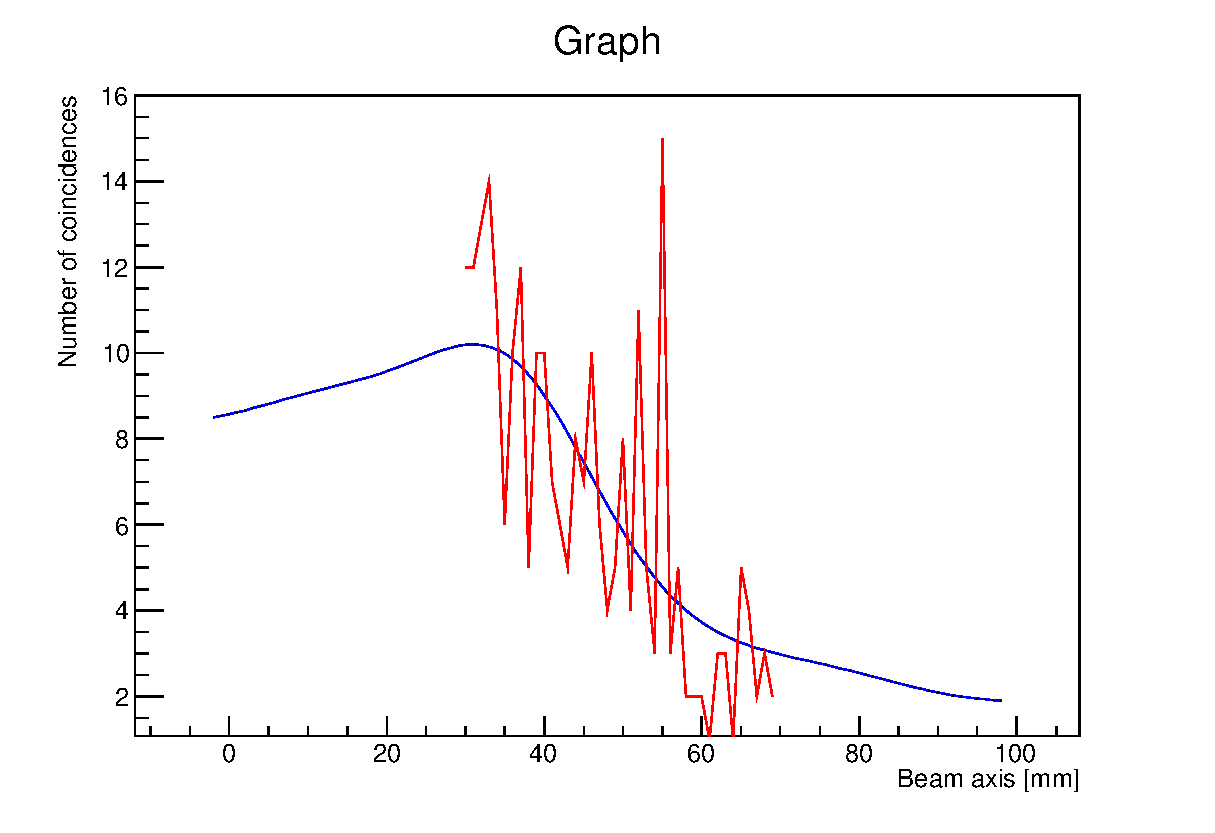
\includegraphics[width=0.33\textwidth]{./Figure/2017-08-02_Nurbs_Poisson_1e8_Article_MLEM.eps}}\\
%  \subfloat[\label{fig:fig_Estimation_Camera_CC_NURBS_Poisson_MLEM}]{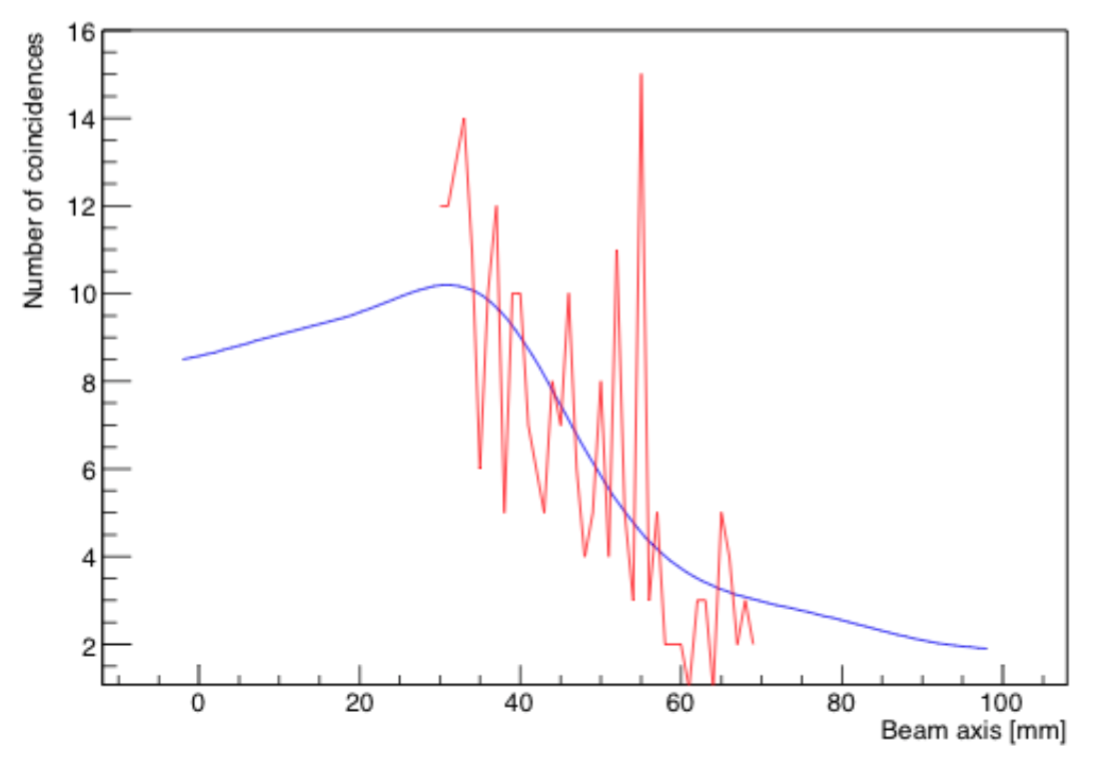
\includegraphics[width=0.33\textwidth]{./Figure/MLEM_NURBS.png}}\\
%   %\subfloat[\label{fig:fig_Results_Chi2_Distribution_Variation_CC_simulation_Hadronth_LC}]{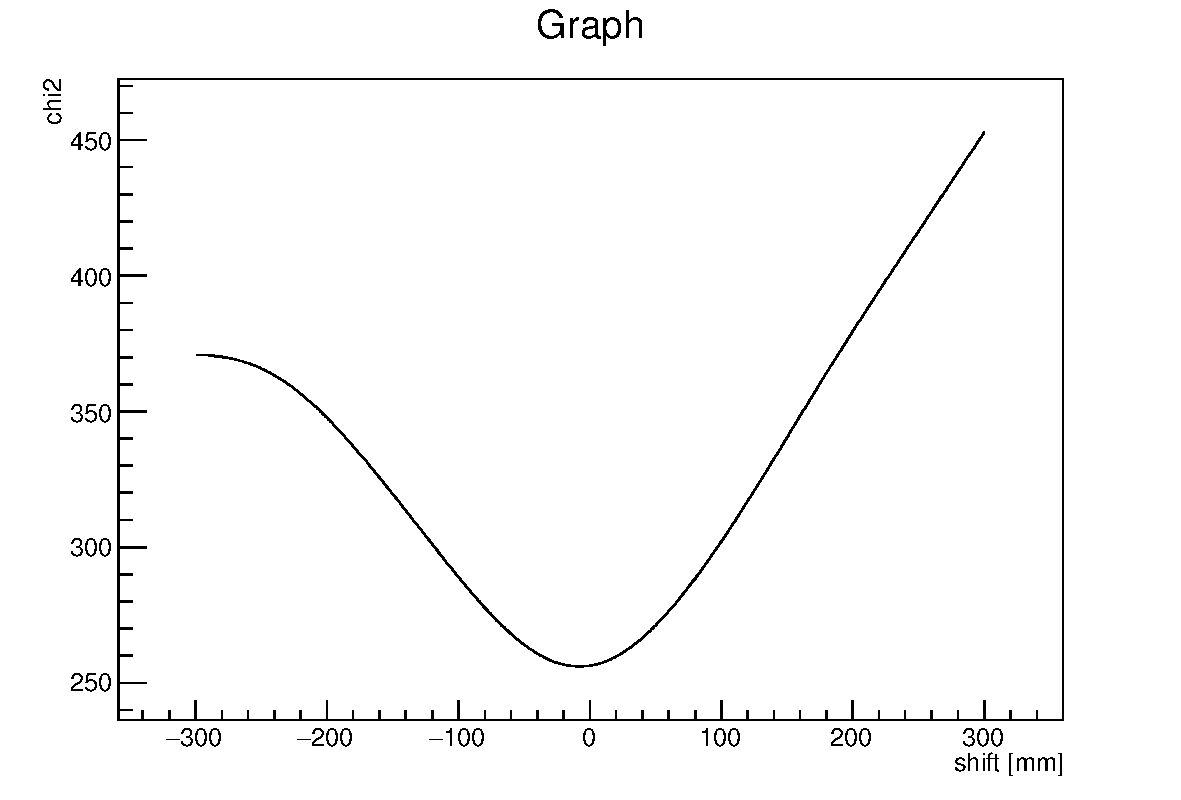
\includegraphics[width=0.33\textwidth]{./Figure/2017-08-02_Distribution_Chi2_1e8_LC.pdf}}
%   \subfloat[\label{fig:fig_Results_Chi2_Distribution_Variation_CC_simulation_Hadronth_LC}]{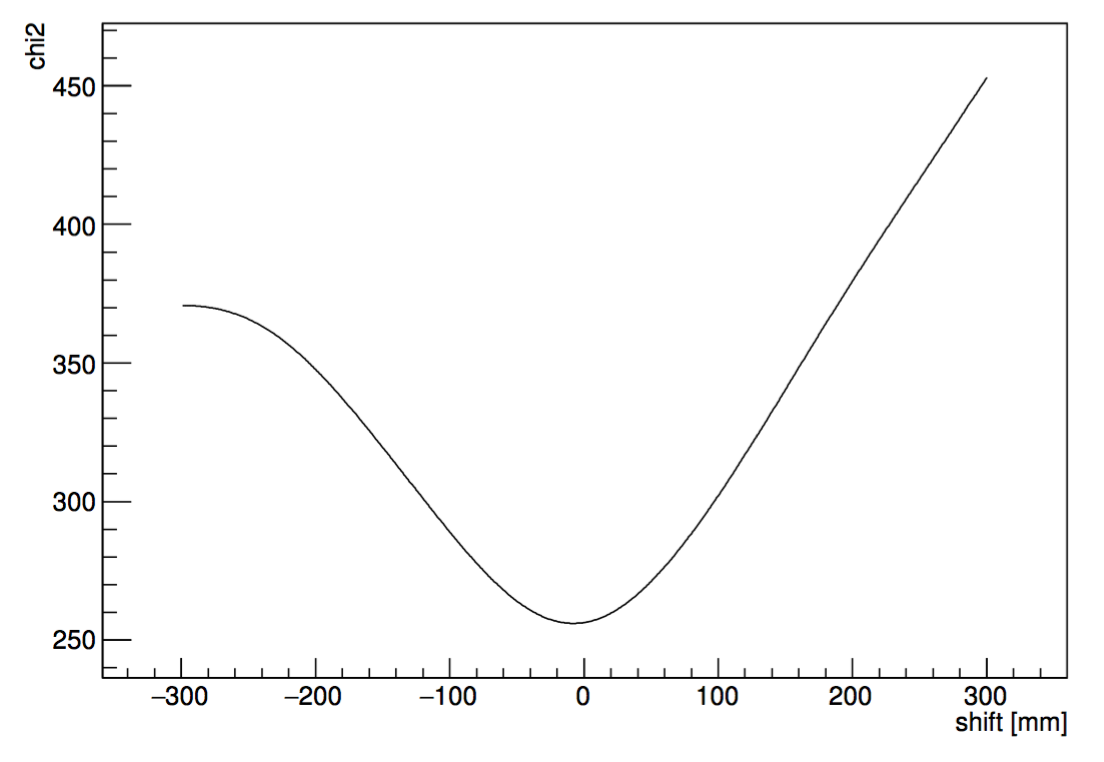
\includegraphics[width=0.33\textwidth]{./Figure/chi2_linecone.png}}
%  %\subfloat[\label{fig:fig_Results_Chi2_Distribution_Variation_CC_simulation_Hadronth_MLEM}]{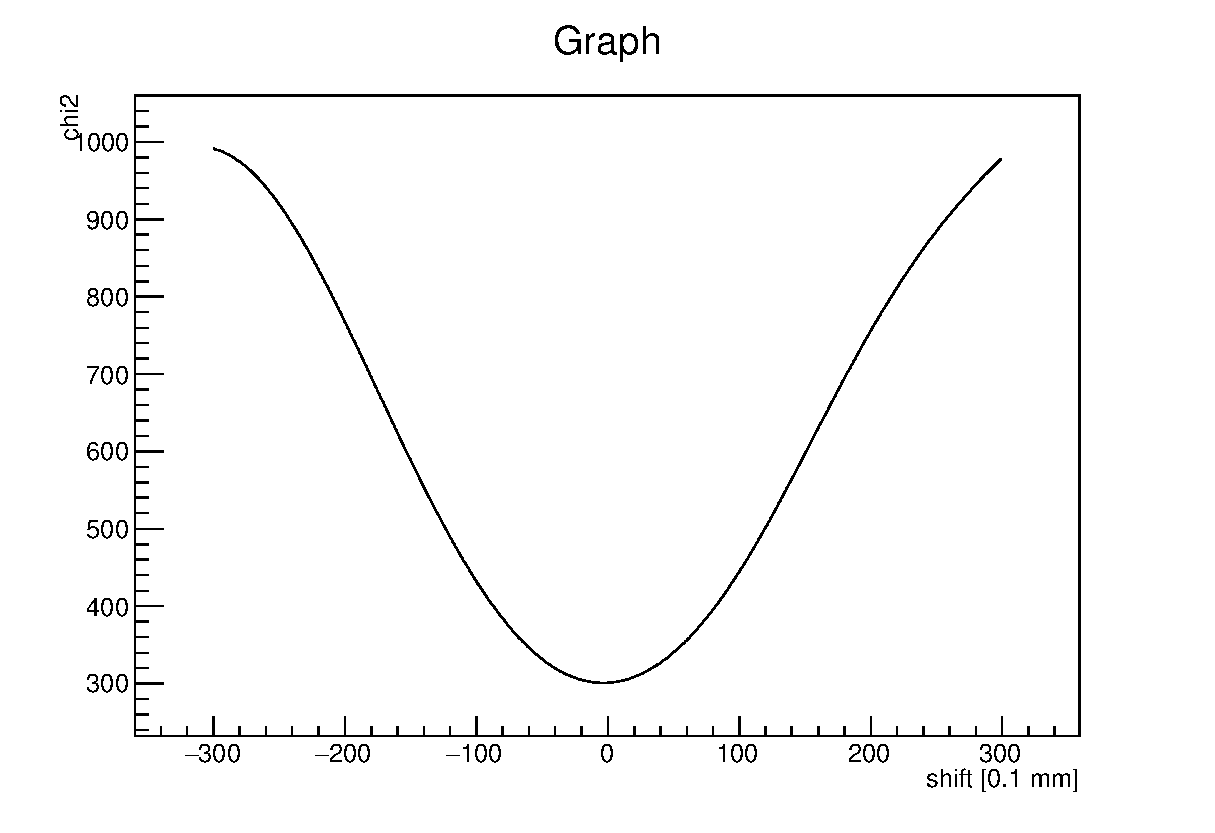
\includegraphics[width=0.33\textwidth]{./Figure/2017-08-02_Distribution_Chi2_Results_binning_1mm_ShiftNurbs0_1mm_1e8_article_MLEM.eps}}\\
%  \subfloat[\label{fig:fig_Results_Chi2_Distribution_Variation_CC_simulation_Hadronth_MLEM}]{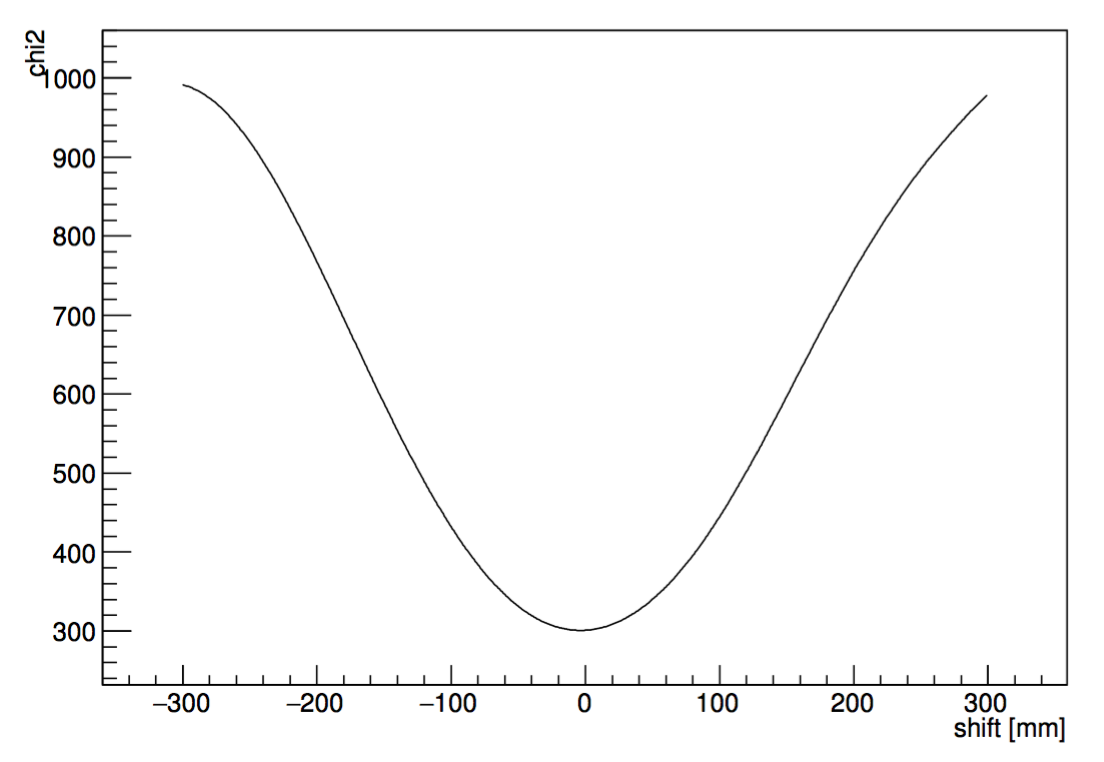
\includegraphics[width=0.33\textwidth]{./Figure/chi2_MLEM.png}}\\
%   %\subfloat[\label{fig:fig_Results_Precision_Distribution_Variation_CC_simulation_Hadronth_LC} ]{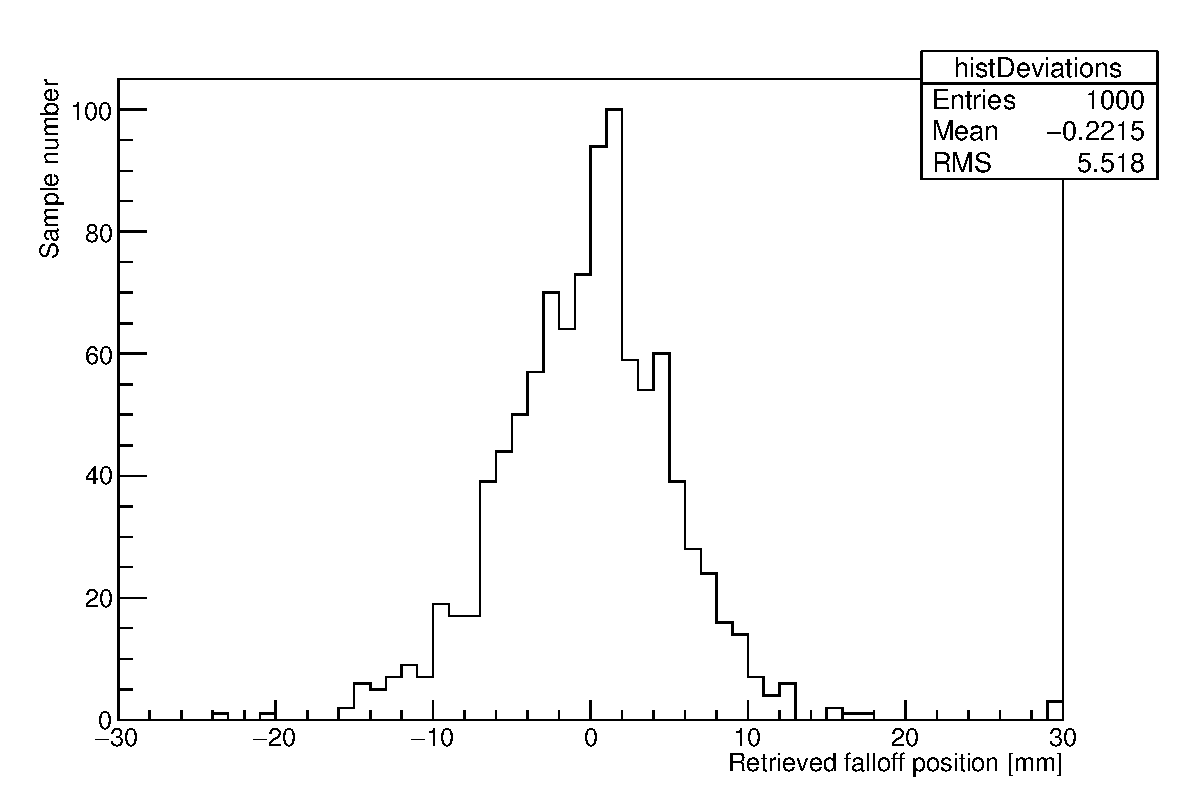
\includegraphics[width=0.33\textwidth]{./Figure/2017-08-02_Distribution_finale_1e8_Article_LC.pdf}}
%   \subfloat[\label{fig:fig_Results_Precision_Distribution_Variation_CC_simulation_Hadronth_LC} ]{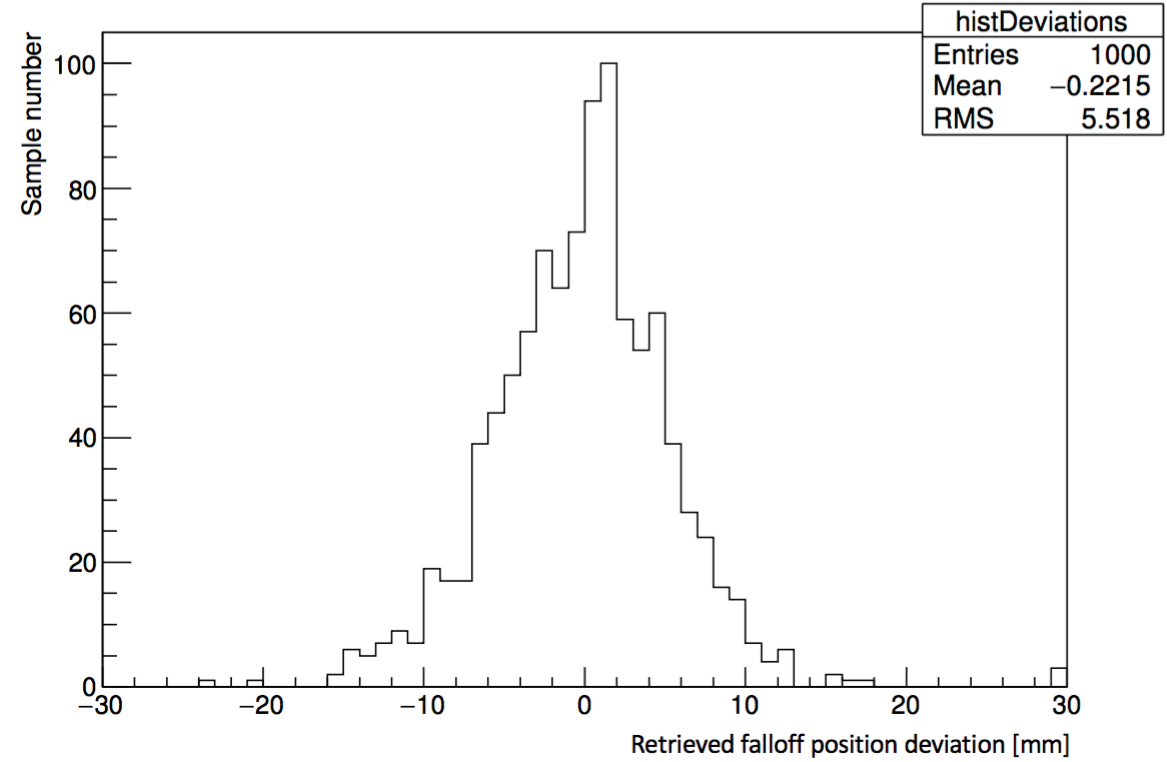
\includegraphics[width=0.33\textwidth]{./Figure/deviation_linecone.png}}
%  %\subfloat[\label{fig:fig_Results_Precision_Distribution_Variation_CC_simulation_Hadronth_MLEM} ]{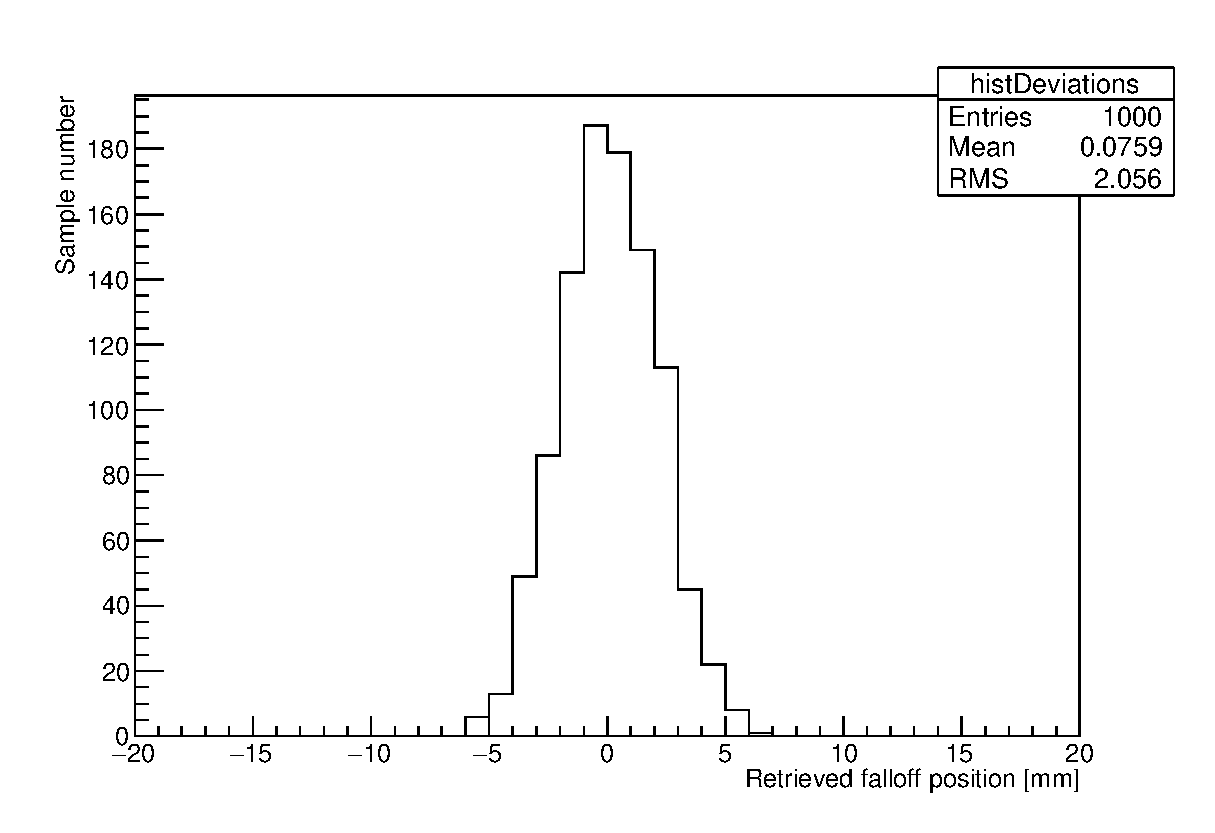
\includegraphics[width=0.33\textwidth]{./Figure/2017-08-02_FallOff_Results_binning_1mm_ShiftNurbs0_1mm_1e8_Article_MLEM.eps}}
%  \subfloat[\label{fig:fig_Results_Precision_Distribution_Variation_CC_simulation_Hadronth_MLEM} ]{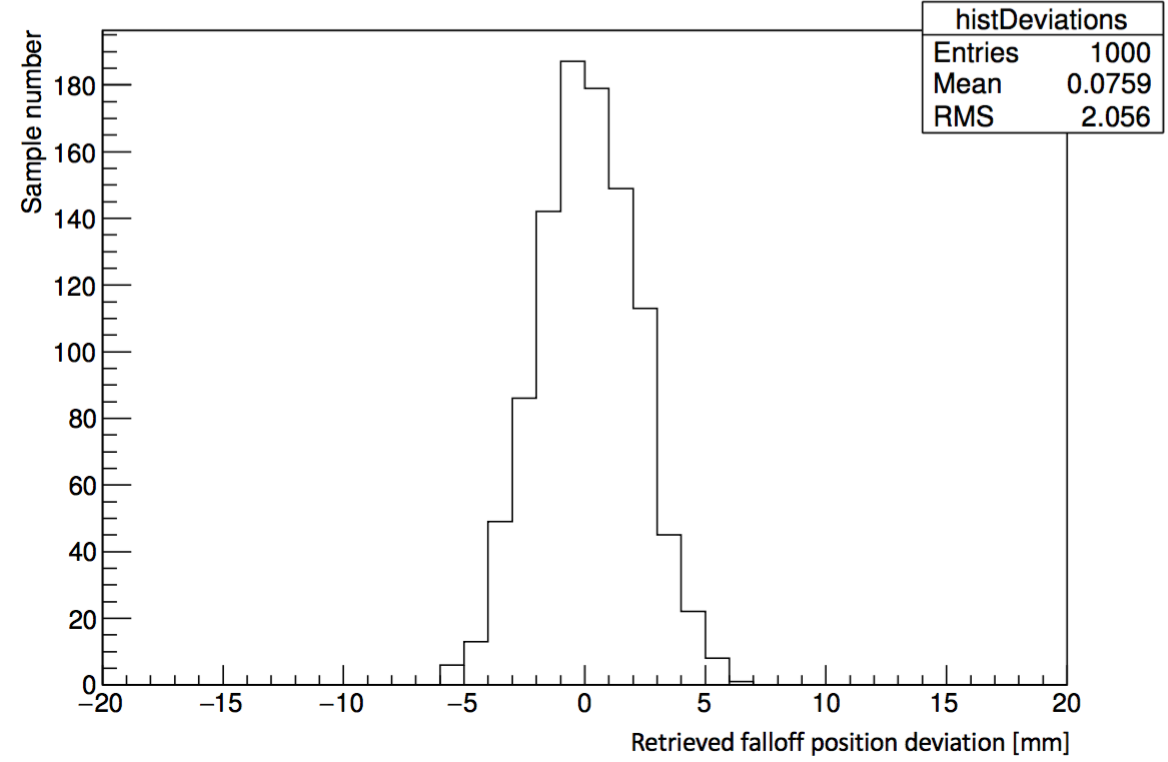
\includegraphics[width=0.33\textwidth]{./Figure/deviation_MLEM.png}}
% \caption{Data processing comparison for the same proton simulation with the line cone algorithm (left column) and the LM-MLEM algorithm (right column). The first row gives the reconstructed profile for $10^{10}$ incident protons. The second row shows the reference curve (blue) and the curve obtained with a $10^8$ incident protons subset. The third row shows the $\chi^2$ distribution for one data subset. The last row represents the distribution of the minimal calculated shifts for 1000 subsets at the same statistics of $10^8$ incident protons.}
% \end{figure}

